\documentclass[12pt,a4paper,onecolumn,openany,twoside]{report}
\usepackage{titletoc}
\renewcommand{\thechapter}{\Roman{chapter}}
\renewcommand{\thesection}{\arabic{section}}
\renewcommand{\thesubsection}{\arabic{section}.\arabic{subsection}}
\renewcommand{\thesubsubsection}{\alph{subsubsection})}

\usepackage[
  inner	=	2.0cm, % Margen interior
  outer	=	2.0cm, % Margen exterior
  top	=	2.0cm, % Margen superior
  bottom=	2.0cm, % Margen inferior
]{geometry}
\usepackage{longtable}
\usepackage{multirow}
\usepackage[framemethod=TikZ]{mdframed}
\renewcommand{\baselinestretch}{1.2} 
\usepackage{amsmath,amsfonts,amssymb}
\usepackage{yfonts}
%%%%%%%%%%%%%%%%%%%%%%%%%%%%%%%%%%%%%%%%%%%%%%%%%%%%%%%%%%%%%%%%%%%%%%
\usepackage{listings}
\usepackage{xcolor}

\definecolor{codegreen}{rgb}{0,0.6,0}
\definecolor{codegray}{rgb}{0.5,0.5,0.5}
\definecolor{codepurple}{rgb}{0.58,0,0.82}
\definecolor{backcolour}{rgb}{0.90,0.90,0.90}

\lstdefinestyle{mystyle}{
    backgroundcolor=\color{backcolour},   
    commentstyle=\color{codegreen},
    keywordstyle=\color{magenta},
    numberstyle=\tiny\color{codegray},
    stringstyle=\color{codepurple},
    basicstyle=\ttfamily\footnotesize,
    breakatwhitespace=false,         
    breaklines=false,
    captionpos=b,                    
    keepspaces=true,                 
    numbers=left,                    
    numbersep=10pt,                  
    showspaces=false,                
    showstringspaces=false,
    showtabs=false,                  
    tabsize=4
}

\lstset{style=mystyle,}
%%%%%%%%%%%%%%%%%%%%%%

\usepackage{algorithm}
\usepackage{algpseudocode}
\usepackage{caption}
\DeclareCaptionFormat{myformat}{#3}
\captionsetup[algorithm]{format=myformat}
\renewcommand{\algorithmicrequire}{\textbf{Input:}}
\renewcommand{\algorithmicensure}{\textbf{Output:}}
\renewcommand{\algorithmicfunction}{\textbf{procedure}}
\newcommand{\algorithmicendfunction}{\algorithmicend\ \algorithmicfunction}
\renewcommand{\algorithmiccomment}[1]{ // #1}
\definecolor{cmt}{RGB}{87,180,74}

%%%%%%%%%%%%%%%%%%%%%%%%
\usepackage{setspace} 
\usepackage[utf8]{inputenc}
\usepackage[vietnamese]{babel}
\usepackage[hidelinks]{hyperref} 
\usepackage{lipsum}
\usepackage{colortbl}
\usepackage{multirow}
\usepackage{multicol}
\usepackage{fancyhdr}
\usepackage{titlesec}
\usepackage{enumitem}
\usepackage{listings}
\usepackage{amsthm}
\usepackage{array}
\usepackage{cases} 
\usepackage{graphicx}

\setlength{\parindent}{0pt}
\usepackage{xcolor}
\usepackage{tikz} 
\usepackage{scrextend}

\usetikzlibrary{calc}
\usepackage{comment}
\renewcommand{\thefigure}{\arabic{figure}}
%%%%%%%%%%%%%%%%% 

\usepackage{tikz}
\usetikzlibrary{decorations.pathreplacing,calc}
\newcommand{\tikzmark}[1]{\tikz[overlay,remember picture] \node (#1) {};}

\newcommand*{\SpaceReservedForComments}{2.5cm}%
\newcommand*{\HorizontalOffset}{-0.5em}%
\newcommand*{\VerticalOffset}{0.7ex}%
\newcommand*{\AddNote}[4][]{%
    %% #1 = draw options
    %% #2 = top line number to start comment from
    %% #3 = bottom line number where comment ends
    %% #4 = text of comment
    \begin{tikzpicture}[overlay, remember picture]
        \draw [decoration={brace,amplitude=0.5em},decorate,ultra thick,red, #1]
            ($(#3)+(\HorizontalOffset,-\VerticalOffset)$) --  ($(#2)+(\HorizontalOffset,\VerticalOffset)$)
            node [align=left, text width=\SpaceReservedForComments-1.0em, pos=0.5, anchor=east] {#4};
    \end{tikzpicture}
}%

\makeatletter% Add a \tkizmark for each line so we can reference it later
    \algrenewcommand\alglinenumber[1]{\tikzmark{\arabic{ALG@line}}\tiny#1:}
\makeatother

%%%%%%%%%%%%%%%%% 
\usetikzlibrary{shapes.multipart}

\tikzset{block/.style={
        font=\sffamily,
        draw=black,
        thin,
        fill=pink!50,
        rectangle split,
        rectangle split horizontal,
        rectangle split parts=#1,
        outer sep=0pt},
        %
        gblock/.style={
            block,
            rectangle split parts=#1,
            fill=green!30}
        }
%%%%%%%%%%%%%%%%%%%%
\usepackage{tocloft}

\setlength{\cftbeforesecskip}{2pt}
\setlength{\cftbeforechapskip}{3pt}
\setlength{\cftbeforepartskip}{8pt}
\usepackage{subcaption}
\usepackage[table]{xcolor}

\begin{document}

\setcounter{tocdepth}{1}
\renewcommand\cftchapfont{\Large\bfseries}
\renewcommand\cftsecfont{\large}

\renewcommand\cftchapafterpnum{\par\addvspace{8pt}}
\renewcommand\cftsecafterpnum{\par\addvspace{6pt}}
\cftsetindents{chapter}{1em}{3em}

\begin{titlepage}
%\SetWatermarkText{\includegraphics[width = 0.97\paperwidth,
%height = 0.97\paperheight]{bia.png}}
%\SetWatermarkAngle{0} 
%\SetWatermarkText{\includegraphics[scale=1]{hust.png}}
%\SetWatermarkAngle{0} 
\begin{tikzpicture}[remember picture,overlay,inner sep=0,outer sep=0]
     \draw[blue!40!black,line width=4pt] ([xshift=-1.5cm,yshift=-2cm]current page.north east) coordinate (A)--([xshift=1.5cm,yshift=-2cm]current page.north west) coordinate(B)--([xshift=1.5cm,yshift=2cm]current page.south west) coordinate (C)--([xshift=-1.5cm,yshift=2cm]current page.south east) coordinate(D)--cycle;
     
     \draw ([yshift=0.5cm,xshift=-0.5cm]A)-- ([yshift=0.5cm,xshift=0.5cm]B)--
     ([yshift=-0.5cm,xshift=0.5cm]B) --([yshift=-0.5cm,xshift=-0.5cm]B)--([yshift=0.5cm,xshift=-0.5cm]C)--([yshift=0.5cm,xshift=0.5cm]C)--([yshift=-0.5cm,xshift=0.5cm]C)-- ([yshift=-0.5cm,xshift=-0.5cm]D)--([yshift=0.5cm,xshift=-0.5cm]D)--([yshift=0.5cm,xshift=0.5cm]D)--([yshift=-0.5cm,xshift=0.5cm]A)--([yshift=-0.5cm,xshift=-0.5cm]A)--([yshift=0.5cm,xshift=-0.5cm]A);


     \draw ([yshift=-0.3cm,xshift=0.3cm]A)-- ([yshift=-0.3cm,xshift=-0.3cm]B)--
     ([yshift=0.3cm,xshift=-0.3cm]B) --([yshift=0.3cm,xshift=0.3cm]B)--([yshift=-0.3cm,xshift=0.3cm]C)--([yshift=-0.3cm,xshift=-0.3cm]C)--([yshift=0.3cm,xshift=-0.3cm]C)-- ([yshift=0.3cm,xshift=0.3cm]D)--([yshift=-0.3cm,xshift=0.3cm]D)--([yshift=-0.3cm,xshift=-0.3cm]D)--([yshift=0.3cm,xshift=-0.3cm]A)--([yshift=0.3cm,xshift=0.3cm]A)--([yshift=-0.3cm,xshift=0.3cm]A);

\end{tikzpicture}

\begin{center}
    \vspace{6pt}
    
    \textbf{ĐẠI HỌC QUỐC GIA THÀNH PHỐ HỐ CHÍ MINH}\\
    \textbf{TRƯỜNG ĐẠI HỌC KHOA HỌC TỰ NHIÊN}
\end{center}
\vspace{8pt}
\begin{center}
    
\includegraphics[scale=0.6]{pic/hcmus.png}
    
    \vspace{12pt}
    
     \fontsize{14pt}{17pt}\selectfont  
    \textbf{CẤU TRÚC DỮ LIỆU VÀ GIẢI THUẬT}
\end{center}
\begin{flushleft}
    \fontsize{14pt}{17pt}\selectfont  
    \textbf{\textsl{ĐỀ TÀI}}
\end{flushleft}
\begin{center}
    \fontsize{19pt}{17pt}\selectfont 
    \textbf{\textrm{CÁC THUẬT TOÁN TÌM KIẾM TRÊN ĐỒ THỊ}}
\end{center}
\vspace{14pt}
 \fontsize{13pt}{17pt}\selectfont  
 \hspace{2cm}
\textbf{Nhóm sinh viên thực hiện:}
\begin{center}
\begin{tabular}{p{0.3\textwidth}p{0.15\textwidth}p{0.15\textwidth}}
 {\it \textbf{Họ và tên}} & {\it \textbf{MSSV}} & {\it \textbf{Lớp}} \\ 
 Nguyễn Đặng Anh Thư & 21280111 & 21KDL1B \\  
 Nguyễn Nhật Minh Thư & 21280112 & 21KDL1B  \\
 & & \\ \\
\end{tabular}
\end{center}

\begin{center}
    \vspace{17pt}
    \textbf{TP.Hồ Chí Minh, 12 - 2022}
\end{center}


\end{titlepage}

\tableofcontents
\newpage
\chapter*{\centering Lời mở đầu}\addcontentsline{toc}{chapter}{Lời mở đầu}

\hspace{0.42cm}
Lời đầu tiên, chúng em xin bày tỏ sự tôn trọng và biết ơn tới thầy Nguyễn Bảo Long - giảng viên phần Thực hành bộ môn Cấu trúc dữ liệu \& giải thuật lớp 21KDL1 đã tạo cơ hội cho chúng em được học tập thông qua đồ án và giải đáp những thắc mắc của chúng em trong quá trình thực hiện.\\

\hspace{0.42cm}
Các thuật toán tìm kiếm trên đồ thị là một vấn đề cơ bản trong cấu trúc dữ liệu và thiết kế thuật toán. Mặc dù để giải quyết chung cho một bài toán thế nhưng để áp dụng cho từng trường hợp và từng bộ dữ liệu khác nhau (đồ thị vô hướng, đồ thị có hướng, đồ thị có trọng số âm, đồ thị có trọng số không âm,...), rất nhiều thuật toán tìm kiếm trên đồ thị đã được phát triển với đa dạng cách tiếp cận. Trong đồ án này, chúng em sẽ trình bày về ý tưởng, cách cài đặt và thời gian thực hiện của tổng cộng 5 thuật toán, cụ thể là Depth First Search, Breadth First Search, Uniform Cost Search, Greedy Best First Search và A* Search. \\

\hspace{0.42cm}
Chúng em cam kết rằng đây là thành quả nghiên cứu của riêng chúng em chứ không sao chép từ bất kỳ nguồn nào.\\


\begin{minipage}{0.5\textwidth}
\hspace{6cm} \ 
\end{minipage}
\begin{minipage}{0.4\textwidth}
    \begin{center}
    \textbf{Ký tên}\\ \ \\ \ \\

\textbf{Nguyễn Nhật Minh Thư}\\
\textbf{Nguyễn Đặng Anh Thư}
    \end{center}
\end{minipage}

\chapter*{\vspace{-3cm} \centering Phân công công việc và đánh giá}\addcontentsline{toc}{chapter}{Phân công công việc và đánh giá}
\vspace{-1cm}
\begin{table}[H]
{
\centering
\extrarowheight = -0.25ex
\renewcommand{\arraystretch}{1.5}
\begin{tabular}{|m{1.5cm}|m{6.6cm}|m{2.4cm}|m{2cm}|m{2.7cm}|}
\hline
\rowcolor[RGB]{229,229,229} \begin{center}\textbf{Công việc}\end{center}& \centering\textbf{Mô tả công việc} & \centering\textbf{Thời gian} & \centering\textbf{Người thực hiện} & \begin{center}\textbf{Đánh giá\\(Thang 10)}\end{center} \\ \hline
   & - Tìm hiểu về thuật toán DFS, BFS, Greedy: Ý tưởng chung, mã giả, nhận xét và ví dụ \par
           - So sánh thuật toán DFS và BFS \par So sánh Uniformed và Informed Search & 24/11 - 30/11 & Anh Thư & \begin{center} 10 \end{center}\\ \cline{2-5}
    \centering Report & Tìm hiểu về thuật toán UCS, A*: Ý tưởng chung, mã giả, nhận xét và ví dụ \par
    - So sánh thuật toán Dijkstra, UCS \par So sánh Uniformed và Informed Search & 24/11 - 30/11 & Minh Thư & \begin{center} 10 \end{center} \\ \cline{2-5}
   & Viết báo cáo bằng Latex: \par
   - Trang bìa, mục lục, lời cảm ơn, lời kết, tham khảo \par
   - Tự trình bày lại phần tìm hiểu và so sánh được giao \par
   - Nhận xét và mô tả ngắn gọn quá trình tìm kiếm của thuật toán
   & 1/12 - 8/12 & Cả nhóm & \begin{center} 10 \end{center} \\ \hline
   \centering \textcolor{white}{t} \par \textcolor{white}{t} \par \textcolor{white}{t} \par \textcolor{white}{t} \par Cài đặt\par(Code) & Cài đặt thuật toán DFS và BFS: \par
           - Tìm đường đi giữa 2 node cho trước trong đồ thị \par
           - Cài đặt thông qua current, open\_set và closed\_set & 1/12 - 7/12 & Anh Thư & \begin{center} 10 \end{center} \\ \cline{2-5}
                     & Cài đặt thuật toán UCS \& A* \& Greedy: \par
           - Tìm đường đi giữa 2 node cho trước trong đồ thị \par
           - Cài đặt thông qua current, open\_set và closed\_set  & 1/12 - 7/12 & Minh Thư & \begin{center} 10 \end{center} \\ \hline
   \begin{center} Video \end{center} & - Video được phân đoạn quay quá trình chạy thuật toán\par
                - Video mỗi thuật toán không quá 3 phút \par
                - Upload Youtube và để đính kèm link trong file link.txt & 8/12 - 9/12 & Cả nhóm & \begin{center} 10 \end{center} \\ \hline
                \multicolumn{4}{|c}{Đánh giá tổng quan} & \multicolumn{1}{|c|}{10}  \\ \hline
\end{tabular}\par
}
\caption{Bảng kế hoạch và phân công công việc đồ án}
\end{table}

\chapter{Tìm hiểu và trình bày các thuật toán tìm kiếm trên đồ thị}

\section{Depth First Search}
\subsection{Ý tưởng chung}
\hspace{0.42cm}Thuật toán DFS sẽ ưu tiên duyệt theo chiều “sâu”. Bắt đầu từ đỉnh nguồn, DFS sẽ duyệt các đỉnh thuộc cùng một nhánh đến khi không thể đi xa hơn được nữa, thì mới chuyển sang duyệt nhánh tiếp theo (backtracking). Thuật toán cứ tiếp tục đến khi tìm được đường đi đến đỉnh đích. Thuật toán này sử dụng chiến lược Last In First Out (LIFO) và do đó nó được cài đặt bằng cách sử dụng ngăn xếp (stack).
\subsection{Mã giả}
\begin{algorithm}[H]
    \caption{\textbf{Mã giả:} Depth First Search}
    \begin{algorithmic}[1]
    \Require{
    \begin{tabular}{cl}
    G & Đồ thị cần tìm đường đi\\
    start & Đỉnh bắt đầu\\
    goal & Đỉnh đích\\
    \end{tabular}
    }
    \Ensure{ \begin{tabular}{cl}
    Path & Đường đi từ start tới goal (nếu có)\\
    \end{tabular}} 
      \Function{DFS}{$G,start,goal$}
        \State $open\_set \gets \text{Stack}$ \textcolor{cmt}{\Comment{ First In Last Out}}
        \State \textcolor{cmt}{\Comment{ Inserting start in stack until all its neighbour vertices are marked}}
        \State \text{$open\_set$.$\textbf{push}($ $start$ $ )$}
        \While{$open\_set$ is not empty}
            \State \textcolor{cmt}{\Comment{  Removing that vertex from stack, whose neighbour will be visited now}}
            \State $current \gets open\_set.$\textbf{pop}$( )$
            \State mark $current$ as $closed$
             \If{$current$ is $goal$} 
                    \State \textbf{return} \text{Path}
            \EndIf
            \State \textcolor{cmt}{\Comment{ Processing all the neighbours of current}}
     \algstore{1}
    \end{algorithmic}
\end{algorithm}
\begin{algorithm}[H]
    \begin{algorithmic}[1]
    \algrestore{1}
            \For{\text{each neighbor $w$ of $current$ in $G$} }
                \If{$w$ is \textbf{not in} $closed$} 
                    \State \text{$open\_set$.$\textbf{push}( $ $w$ $ )$}
                \EndIf
            \EndFor
        \EndWhile
        \State \textbf{return} \text{Not found path}
        \EndFunction  
    \end{algorithmic}
\end{algorithm}

\subsection{Nhận xét}
\subsubsection{a) Tính đầy đủ}
\hspace{0.42cm}Tính chất này của DFS phụ thuộc hoàn toàn vào cách cài đặt theo graph-search hay tree-search của thuật toán. Sự khác biệt cơ bản giữa graph-search và tree-search là graph-search có thêm một mảng phụ để lưu trữ những node đã được \textbf{“thăm”} (closed set) còn tree-search thì không. 
\begin{itemize}
    \item Trong tree-search (không có closed set), khi đó thuật toán DFS sẽ không quan tâm là node hiện tại (current node) đã được thăm hay chưa, mà DFS chỉ tiến hành đi càng sâu xuống $\rightarrow$ có thể dẫn tới vòng lặp vô tận $\rightarrow$ không đầy đủ
    \item Trong graph-search (có closed set), đánh dấu các node đã được thăm để tránh tình trạng thăm vô tận như trên $\rightarrow$ đầy đủ
\end{itemize}
\subsubsection{b) Tính tối ưu}
\hspace{0.42cm}Thuật toán DFS không có tính tối ưu đối với cả hai cách cài đặt graph-search và tree-search. Thuật toán chỉ trả về kết quả là đường đi đến đỉnh đích đầu tiên mà nó tìm thấy, mà đường đi đó có thể không tối ưu. Điều này có thể xảy ra nếu có nhiều hơn một cách đi từ đỉnh nguồn đến đỉnh đích.
\subsubsection{c) Độ phức tạp}
\hspace{0.42cm}Trong trường hợp xấu nhất, DFS phải duyệt hết toàn bộ cây. Vì khi đó node đích cần tìm lại là node lá của nhánh cây được duyệt sau cùng (DFS cài đặt bằng đệ quy thì sẽ là nhánh bên phải, DFS cài đặt khử đệ quy bằng cách xét các node kề thì sẽ là nhánh bên trái).

\hspace{0.42cm}Với \textbf{m} = độ sâu tối đa có thể duyệt từ một node và \textbf{b} = số node tối đa mà 1 node có thể mở rộng. Khi đó độ phức tạp về thời gian là: $T(b)= b^0 + b^1 + b^2 +...+ b^m = O(b^m)$.

\subsection{Ví dụ}

\begin{figure}[H]
    \centering
    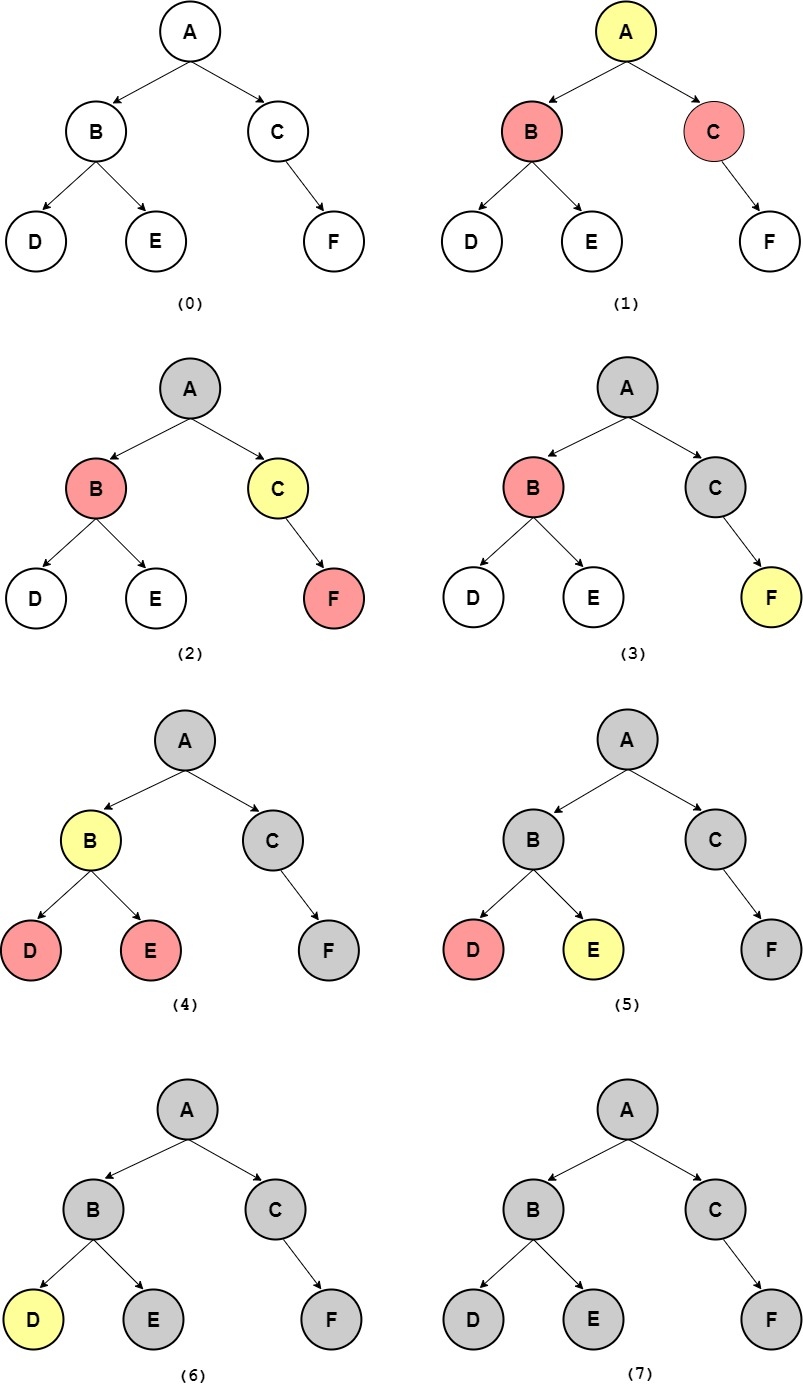
\includegraphics[scale=0.5]{pic/DFS1.jpg}
    \label{fig:my_label}
\end{figure}

\begin{table}[H]
{
\centering
\begin{tabular}{|m{1cm}|m{6.7cm}|m{1.6cm}|m{2.5cm}|m{3cm}|}
\hline
\begin{center}\cellcolor{green!25}\textbf{Step}\end{center}& \centering\cellcolor{green!25}\textbf{Description} & \centering\cellcolor{yellow!25}\textbf{Current} & \centering\cellcolor{red!25}\textbf{Opened Set\\(Stack)} & \begin{center}\cellcolor{gray!25}\textbf{Closed Set}\end{center} \\ \hline
   \centering 0 & push(A) into empty Stack & & \begin{center} A \end{center} & \\ \hline
   \centering 1 & pop()= A, push(B) \& push(C) & \begin{center} A \end{center}& \begin{center}B, C \end{center} &  \\ \hline
   \centering 2 & marked A closed, pop()= C, push(F) & \begin{center} C \end{center}& \begin{center} B, F \end{center} & \begin{center} A \end{center}\\ \hline 
   \centering 3 & marked C closed, pop()= F & \begin{center} F \end{center} & \begin{center} B \end{center} & \begin{center} A, C \end{center} \\ \hline 
   \centering 4 & F closed, pop()= P, push(D), push(E) & \begin{center} B \end{center} & \begin{center} D, E \end{center} & \begin{center} A, C, F \end{center} \\ \hline 
   \centering 5 & marked B closed, pop()= E & \begin{center} E \end{center} & \begin{center} D \end{center} & \begin{center} A, C, F, B \end{center} \\ \hline  
   \centering 6 & marked E closed, pop()= D & \begin{center} D \end{center} &  & \begin{center} A, C, F, B, E \end{center} \\ \hline 
   \centering 7 & \begin{center}Traversal: A - C - F - B - E - D \end{center}&  &  &  \\ \hline 
\end{tabular}
}
\caption*{Các bước duyệt cây bằng Depth First Search}
\end{table}
\hspace{0.42cm}Ví dụ ở đây là cách duyệt toàn bộ cây bằng thuật toán DFS, việc tìm kiếm đi từ node gốc đến node đích thì sẽ khác biệt một chút ở chỗ là khi node đang được duyệt (current) chính là node đích cần tìm thì ta sẽ kết thúc quá trình tìm kiếm ngay mà không cần duyệt tiếp nữa.

\section{Breadth First Search}
\subsection{Ý tưởng chung}
\hspace{0.42cm}Ý tưởng của thuật toán BFS là bắt đầu từ đỉnh nguồn của đồ thị sau đó \textbf{“loang”} dần ra các đỉnh kề (có cạnh nối) với đỉnh nguồn, trước khi loang dần đến những đỉnh kề xa hơn. Những đỉnh nào gần với đỉnh nguồn hơn sẽ được loang tới trước. Thuật toán BFS được cài đặt bằng cách sử dụng hàng đợi (queue).
\subsection{Mã giả}
\begin{algorithm}[H]
    \caption{\textbf{Mã giả:} Breadth First Search}
    \begin{algorithmic}[1]
    \Require{
    \begin{tabular}{cl}
    G & Đồ thị cần tìm đường đi\\
    start & Đỉnh bắt đầu\\
    goal & Đỉnh đích\\
    \end{tabular}
    }
    \Ensure{ \begin{tabular}{cl}
    Path & Đường đi từ start tới goal (nếu có)\\
    \end{tabular}} 
      \Function{BFS}{$G,start,goal$}
        \State $open\_set \gets \text{Queue}$
        \State \textcolor{cmt}{\Comment{ Inserting start in queue until all its neighbour vertices are marked}}
        \State \text{$open\_set$.$\textbf{enqueue}( $ $start$ $ )$}
        \While{$open\_set$ is not empty}
            \State \textcolor{cmt}{\Comment{  Removing that vertex from queue, whose neighbour will be visited now}}
            \State $current \gets open\_set.\textbf{dequeue}( )$
            \State mark $current$ as $closed$
             \If{$current$ is $goal$} 
                    \State \textbf{return} \text{Path}
            \EndIf
            \State \textcolor{cmt}{\Comment{  processing all the neighbours of current}}
            \For{\text{all neighbours $w$ of $current$ in $G$} }
                \If{$w$ is \textbf{not in} $closed$ \textbf{and} $w$ is not $opened$} 
                    \State \text{$open\_set$.$\textbf{enqueue}( $ $w$ $ )$}
            \EndIf
            \EndFor
        \EndWhile
        \State \textbf{return} \text{Not found path}
        \EndFunction
    \end{algorithmic}
\end{algorithm}
\subsection{Nhận xét}
\subsubsection{a) Tính đầy đủ} 
\hspace{0.42cm}Thuật toán Breadth First Search (BFS) có tính đầy đủ, nếu b (= số node tối đa mà 1 node có thể mở rộng được) là hữu hạn. Khi đó BFS sẽ luôn tìm được đường đi từ node nguồn tới node đích, nếu tồn tại đường đi.

\subsubsection{b) Tính tối ưu}
\hspace{0.42cm}Thuật toán BFS về cơ bản là không tối ưu vì nó không xét đến chi phí các cạnh để xác định cần thay thế node nào khi tìm kiếm đường đi. BFS chỉ đảm bảo được tính tối ưu khi đồ thị không có trọng số hoặc tất cả trọng số bằng nhau (chi phí tất cả các cạnh bằng nhau). Khi đó thuật toán này sẽ luôn tìm được đường đi ngắn nhất từ đỉnh nguồn tới đỉnh đích, nếu tồn tại đường đi.

\subsubsection{c) Độ phức tạp}
\hspace{0.42cm}Trong trường hợp xấu nhất thì node đích là node cuối cùng được duyệt ở độ sâu \textbf{d}. Vậy nên  BFS sẽ phải duyệt hết tất cả các node từ độ sâu là 0 đến độ sâu của node đích.

\hspace{0.42cm}Với \textbf{d} = độ sâu của node đích và \textbf{b} = số node tối đa mà 1 node có thể mở rộng. Khi đó độ phức tạp về thời gian là: $T(b) = b^0 + b^1 + b^2 + … + b^d + b^{d+1}= O(b^{d+1})$

\hspace{0.42cm}Tại sao lại là $d+1$ ? Vì như trong mã giả đã trình bày, chúng ta xét \textbf{current} có phải là \textbf{goal} hay không khi đã \textit{dequeue} khỏi \textbf{opened\_set}. Cho nên điều này khiến ta phải duyệt thêm một lớp nữa, chính vì vậy độ phức tạp phải là $O(b^{d+1})$ (Về cơ bản thì nó xấp xỉ $O(b^d)$ = Độ phức tạp thời gian như một số tài liệu khác có trình bày).
\subsection{Ví dụ}
\vspace{-0.5cm}
\begin{figure}[H]
    \centering
    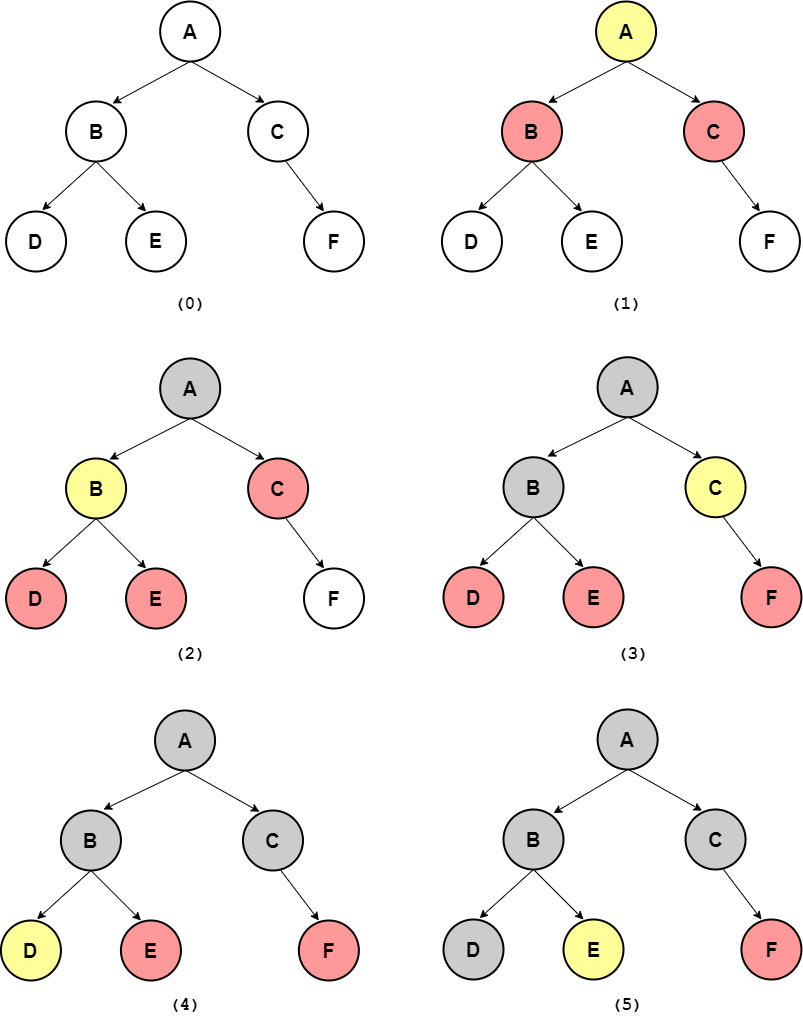
\includegraphics[scale=0.45]{pic/BFS1.png}
    \label{fig:my_label}
\end{figure}
\begin{figure}[H]
    \centering
    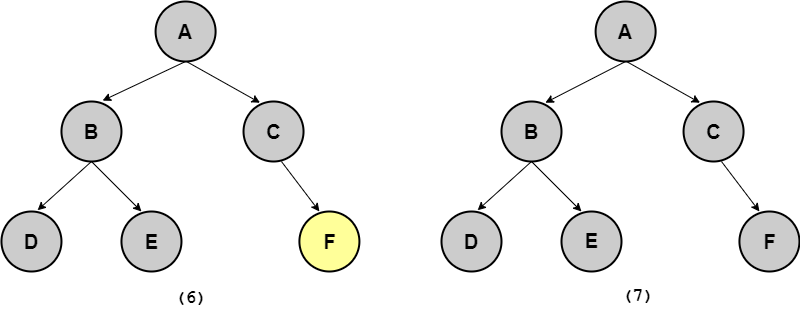
\includegraphics[scale=0.45]{pic/BFS2.png}
    \label{fig:my_label}
\end{figure}
\vspace{-0.8 cm}
\begin{table}[H]
{
\centering
\begin{tabular}{|m{1cm}|m{6.7cm}|m{1.6cm}|m{2.5cm}|m{3cm}|}
\hline
\begin{center}\cellcolor{green!25}\textbf{Step}\end{center}& \centering\cellcolor{green!25}\textbf{Description} & \centering\cellcolor{yellow!25}\textbf{Current} & \centering\cellcolor{red!25}\textbf{Opened Set\\(Queue)} & \begin{center}\cellcolor{gray!25}\textbf{Closed Set}\end{center} \\ \hline
   \centering 0 & enqueue(A) into empty Queue & & \begin{center} A \end{center} & \\ \hline
   \centering 1 & dequeue()= A, enqueue(B),\par enqueue(C) & \begin{center} A \end{center}& \begin{center}B, C \end{center} &  \\ \hline
   \centering 2 & A closed, dequeue()= B,\par enqueue(D), enqueue(E) & \begin{center} B \end{center}& \begin{center} C, D, E \end{center} & \begin{center} A \end{center}\\ \hline 
   \centering 3 & B closed, dequeue()= C, enqueue(F) & \begin{center} C \end{center} & \begin{center} D, E, F \end{center} & \begin{center} A, B \end{center} \\ \hline 
   \centering 4 & C closed, , dequeue()= D & \begin{center} D \end{center} & \begin{center} E, F \end{center} & \begin{center} A, B, C \end{center} \\ \hline 
   \centering 5 & D closed, dequeue()= E & \begin{center} E \end{center} & \begin{center} F \end{center} & \begin{center} A, B, C, D \end{center} \\ \hline  
   \centering 6 & E closed, dequeue()= F & \begin{center} F \end{center} &  & \begin{center} A, B, C, D, E \end{center} \\ \hline 
   \centering 7 & \begin{center}Traversal: A - B - C - D - E - F \end{center}&  &  &  \\ \hline 
\end{tabular}
}
\caption*{Các bước duyệt cây bằng Breadth First Search}
\end{table}
\hspace{0.42cm}Ví dụ ở đây là cách duyệt toàn bộ cây bằng thuật toán BFS, việc tìm kiếm đi từ node gốc đến node đích thì sẽ khác biệt một chút ở chỗ là khi node đang được duyệt (current) chính là node đích cần tìm thì ta sẽ kết thúc quá trình tìm kiếm ngay mà không cần duyệt tiếp nữa.

\section{Uniform Cost Search}
\subsection{Ý tưởng chung}
\hspace{0.42cm}Uniform-cost search (UCS) hay Tìm kiếm chi phí cực tiểu áp dụng thuật toán Dijkstra. Nói qua về thuật toán Dijkstra là một trong những thuật toán cổ điển để giải quyết bài toán tìm đường đi ngắn nhất từ một điểm cho trước tới tất cả các điểm còn lại trong đồ thị có trọng số không âm. Quay trở lại với UCS thì thuật toán này đánh giá chi phí và lựa chọn node tiếp theo với mục tiêu là chi phí đường đi là thấp nhất tính từ node gốc đến node tiếp theo được chọn. Hàm tính chi phí được ký hiệu là  \textbf{$g(x) = $ khoảng cách giữa 2 node}. Quá trình này dừng lại cho đến khi ta tìm được đến node đích.
\subsection{Mã giả}
\begin{algorithm}[H]
    \caption{\textbf{Mã giả:} Uniform Cost Search}
    \begin{algorithmic}[1]
    \Require{
    \begin{tabular}{cl}
    G & Đồ thị cần tìm đường đi\\
    start & Đỉnh bắt đầu\\
    goal & Đỉnh đích\\
    \end{tabular}
    }
    \Ensure{\begin{tabular}{cl}
    Path & Đường đi từ start tới goal (nếu có)\\
    \end{tabular}} 
    \State \textcolor{cmt}{\Comment{Get distance from start to goal by Euclidean distance}}
    \Function{get\_distance}{$start, goal$}
        \State \Return \textbf{sqrt}$((goal.x-start.x)^2+(goal.y-start.y)^2))$
    \EndFunction
    \State \textcolor{cmt}{\Comment{Implement Function}}
    \Function{UCS}{$G,start,goal$}
        \State $open\_set \gets \text{Priority Queue}$ \textcolor{cmt}{\Comment{ (key, value) = (node, cost)}}
        \State \text{$open\_set$.$\textbf{enqueue}( $ $(start, 0$ $ )$}
        \While{$open\_set$ is not empty}
            \State \textcolor{cmt}{\Comment{  Removing node which lowest cost from priority queue}}
            \State $current \gets open\_set.\textbf{dequeue}( )$
             \If{$current$ is $goal$} 
                    \State \textbf{return} \text{Path}
            \EndIf
            \State mark $current$ as $closed$
            \State \textcolor{cmt}{\Comment{  Processing all neighbors of current}}
            \For{\text{each $node$ of $current$'s neighbors}}
                \If{$node$ is \textbf{not in} $closed$ \textbf{and} $node$ is \textbf{not in} $opened$} 
                    \State $open\_set.\textbf{enqueue}( node, cost + \textbf{get\_distance}(current, node)) $
                \Else{\textbf{ if }$node$ is \textbf{in} $opened$ with higher $cost$}
                    \State \text{replace lower $cost$} \textcolor{cmt}{\Comment{ = cost[current] + \textbf{get\_distance}(current, node)}}
                \EndIf
            \EndFor
        \EndWhile
        \State \textbf{return} \text{Not found path}
    \EndFunction
    \end{algorithmic}
\end{algorithm}
\subsection{Nhận xét}
\subsubsection{a) Tính đầy đủ}
Uniform Cost Search có tính đầy đủ khi đồ thị có trọng số là không âm.  Nếu tồn tại đường đi có chi phí hữu hạn từ đỉnh nguồn đến đỉnh đích, UCS luôn trả về được kết quả là đường đi đó, hơn nữa chi phí của đường đi này sẽ là ngắn nhất vì trong quá trình tìm kiếm đường đi UCS luôn duyệt hết tất cả các khả năng có thể và chọn ra đỉnh có chi phí nhỏ nhất để mở rộng. 
\subsubsection{b) Tính tối ưu}
Uniform Cost Search (UCS) cũng có tính tối ưu khi trọng số tất cả các cạnh của đồ thị là không âm. Từ đỉnh nguồn, UCS sẽ mở rộng dần từng đỉnh trong đường đi bằng cách xét hết tất cả các đỉnh có thể đi và chọn ra đỉnh có tổng chi phí từ đỉnh nguồn đến đỉnh đó thấp nhất để mở rộng. Và khi trọng số tất cả các cạnh là không âm, thì chi phí đường đi đang xét sẽ ngày càng tăng dần, khi đó với chiến lược giải quyết như trên UCS sẽ đảm bảo trả về được đường đi với chi phí nhỏ nhất từ đỉnh nguồn tới đỉnh đích (nếu tồn tại đường đi). Chiến lược được sử dụng trong UCS cũng giống với chiến lược của thuật toán Dijkstra, sự khác biệt chính là UCS sẽ kết thúc khi tìm thấy đường đi ngắn nhất từ đỉnh nguồn tới đỉnh đích và tất cả những đỉnh đã được xét thay vì tìm thấy đường đi ngắn nhất từ đỉnh nguồn đến tất cả các đỉnh còn lại trong đồ thị.
\subsubsection{c) Độ phức tạp}
\hspace{0.42cm}Uniform Cost Search không quan tâm đến tổng số bước của đường đi mà UCS chỉ quan tâm đến tổng chi phí của đường đi, vì vậy không thể đánh giá độ phức tạp của UCS chỉ dựa trên b (= số node tối đa mà 1 node có thể mở rộng) và d (= độ sâu của node đích). Thay vào đó, gọi: 
\begin{itemize}
    \item C* là chi phí đường đi tối ưu
    \item $\epsilon$ là chi phí tối thiểu cho mỗi lần mở rộng 
\end{itemize}
\hspace{0.42cm} Khi đó, độ phức tạp của UCS trong trường hợp xấu nhất là $O(b^{1 + \lfloor C*/\epsilon \rfloor})$ = $O(b^{d+1})$ khi chi phí tất cả các cạnh là bằng nhau.

\subsection{Ví dụ}
\vspace{-0.5cm}
\begin{figure}[H]
    \centering
    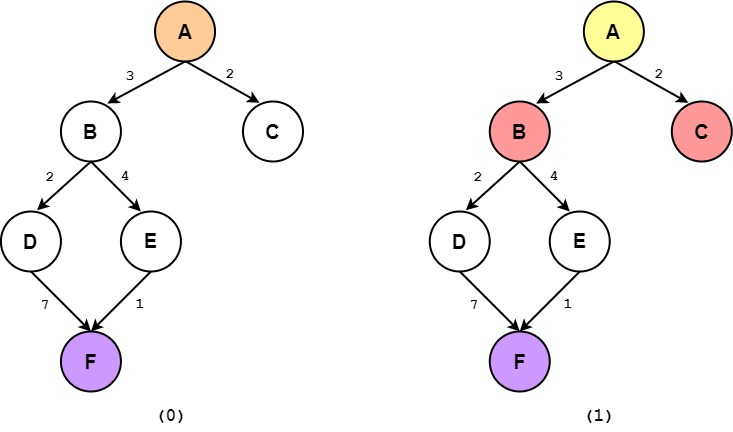
\includegraphics[scale=0.5]{pic/UCS2.jpg}
    \label{fig:my_label}
\end{figure}
\begin{figure}[H]
    \centering
    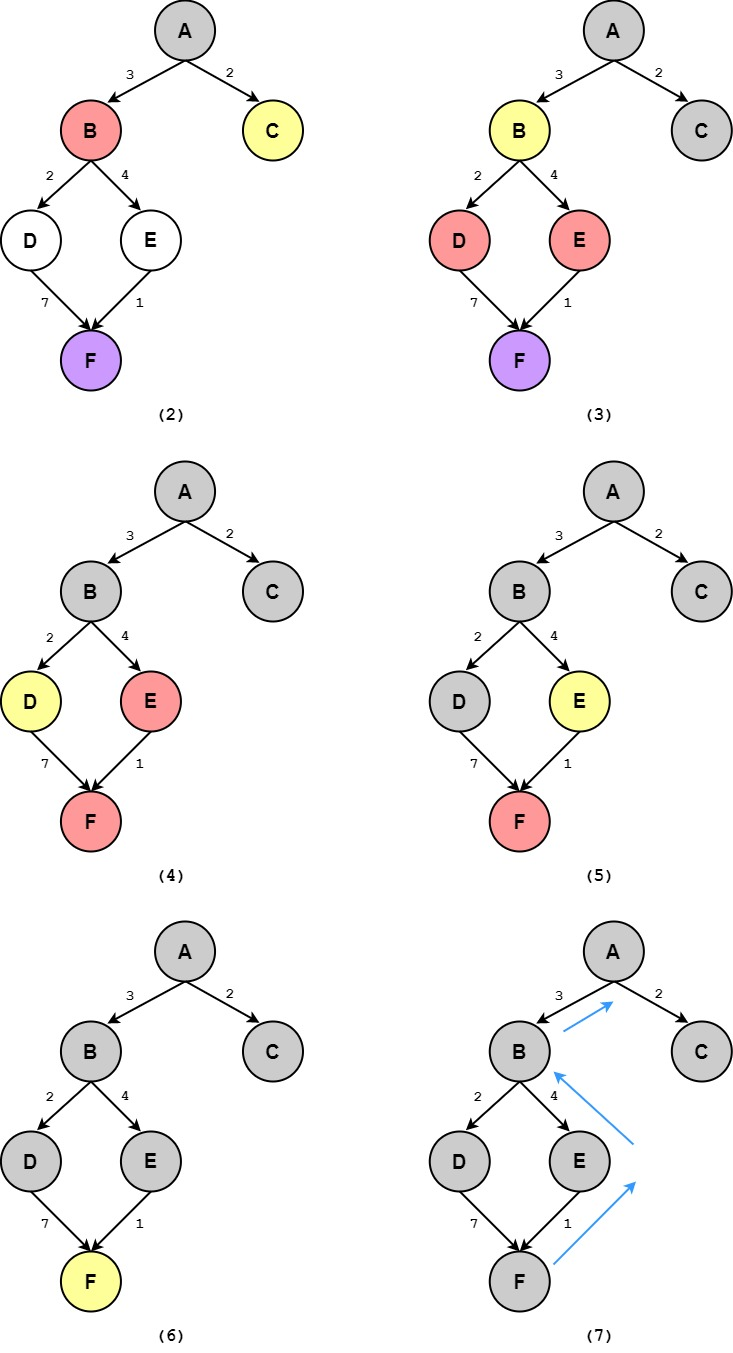
\includegraphics[scale=0.5]{pic/UCS1.jpg}
    \label{fig:my_label}
\end{figure}

\begin{table}[H]
{
\renewcommand{\arraystretch}{1}
\centering
\begin{tabular}{|m{1cm}|m{6.4cm}|m{1.6cm}|m{2.6cm}|m{3.3cm}|}
\hline
\begin{center}\cellcolor{green!25}\textbf{Step}\end{center}& \centering\cellcolor{green!25}\textbf{Description} & \centering\cellcolor{yellow!25}\textbf{Current} & \centering\cellcolor{red!25}\textbf{Opened Set\\(Priority Queue)} & \begin{center}\cellcolor{gray!25}\textbf{Closed Set}\end{center} \\ \hline
   \centering 0 & enqueue(A,0) into empty Queue & & \begin{center} \{(A,0)\} \end{center} & \begin{center} \{-\} \end{center} \\ \hline
   \centering 1 & dequeue()= (A,0), enqueue(B,3),\par enqueue(C,2) & \begin{center} (A,0) \end{center}& \begin{center} \{(C,2),(B,3)\} \end{center} &  \begin{center} \{-\} \end{center} \\ \hline
   \centering 2 & A closed, dequeue()= (C,2) & \begin{center} (C,2) \end{center}& \begin{center} \{(B,3)\} \end{center} & \begin{center} \{(A,0)\} \end{center}\\ \hline 
   \centering 3 & C closed, dequeue()= (B,3),\par enqueue(D,3+2), enqueue(E,3+4) & \begin{center} (B,3) \end{center} & \begin{center} \{(D,5),(E,7)\} \end{center} & \begin{center} \{(A,0),(C,2)\} \end{center} \\ \hline 
   \centering 4 & B closed, dequeue()= (D,5) \par enqueue(F,5+7) & \begin{center} (D,5) \end{center} & \begin{center} \{(E,7),(F,12)\} \end{center} & \begin{center} \{(A,0),(C,2),(B,3)\} \end{center} \\ \hline 
   \centering 5 & D closed, dequeue()= (E,7), \par replace (F,12) with (F,7+1) & \begin{center} (E,7) \end{center} & \begin{center} \{(F,8)\} \end{center} & \begin{center} \{(A,0),(C,2),(B,3),\par(D,5)\} \end{center} \\ \hline  
   \centering 6 & E closed, dequeue()= (F,8) = \textbf{goal}\par Return Path & \begin{center} (F,8) \end{center} &  & \begin{center} \{(A,0),(C,2),(B,3),\par(D,5),(E,7)\} \end{center} \\ \hline 
   \centering 7 & \begin{center}Path A $\rightarrow$ F: A $\rightarrow$ B $\rightarrow$ E $\rightarrow$ F \end{center}&  &  &  \\ \hline 
\end{tabular}
}
\caption*{Các bước tìm kiếm bằng Uniform Cost Search}
\end{table}
\hspace{0.42cm} Để dễ hình dung về ví dụ trên, ta cần lưu ý một số điểm như sau:
\begin{itemize}
    \item \textbf{Opened Set} được cài đặt bằng Priority Queue với phần tử có dạng (Vertex, Cost). Mức độ ưu tiên là Min Cost, tức là phần tử có Cost nhỏ nhất trong Priority Queue sẽ được lấy ra (dequeue) trước.
    \item Khi một phần tử đã được xét một (vài) lần không đồng nghĩa với việc sẽ không xét đến nữa như hai thuật toán DFS và BFS. Phần tử đó chỉ không được xét nữa khi được lấy ra (dequeue) từ \textbf{Opened Set}. Việc xét nhiều lần và có thể gán lại Cost vì có thể tồn tại đường đi khác với chi phí thấp hơn chi phí ban đầu được gán.
\end{itemize}

\section{Greedy Best First Search}
\subsection{Ý tưởng chung}
\hspace{0.42cm} Greedy Best First Search là một thuật toán tìm kiếm đồ thị nằm trong nhóm Tìm kiếm dựa trên kinh nghiệm (Informed Search) với chiến lược tìm kiếm dùng tri thức bổ sung từ việc sử dụng các tri thức cụ thể của bài toán.

\hspace{0.42cm} Thuật toán sẽ sử dụng một hàm đánh giá là hàm heuristic $h(x)$ để đánh giá chi phí để đi từ node hiện tại $x$. Trong quá trình tìm kiếm, Greedy best-first search sẽ mở rộng node “có vẻ” gần với node đích (mục tiêu) nhất.

\subsection{Mã giả}
\begin{algorithm}[H]
    \caption{\textbf{Mã giả:} Greedy Best First Search}
    \begin{algorithmic}[1]
    \Require{
    \begin{tabular}{cl}
    G & Đồ thị cần tìm đường đi\\
    start & Đỉnh bắt đầu\\
    goal & Đỉnh đích\\
    \end{tabular}
    }
    \Ensure{\begin{tabular}{cl}
    Path & Đường đi từ start tới goal (nếu có)\\
    \end{tabular}} 
    \State \textcolor{cmt}{\Comment{Get heuristic from start to goal by Euclidean distance}}
    \Function{get\_heuristic}{$node$}
        \State \Return \textbf{sqrt}$((goal.x-node.x)^2+(goal.y-node.y)^2))$
    \EndFunction
    \State \textcolor{cmt}{\Comment{Implement Function}}
    \Function{Greedy}{$G,start,goal$}
        \State $open\_set \gets \text{Priority Queue}$ \textcolor{cmt}{\Comment{ (key, value) = (node, heuristic)}}
        \State \text{$open\_set$.$\textbf{enqueue}( $ $(start, \textbf{get\_heuristic}(start)$ $ )$}
        \While{$open\_set$ is not empty}
            \State \textcolor{cmt}{\Comment{  Removing node which lowest heuristic from priority queue}}
            \State $current \gets open\_set.\textbf{dequeue}( )$
             \If{$current$ is $goal$} 
                    \State \textbf{return} \text{Path}
            \EndIf
            \State mark $current$ as $closed$
            \State \textcolor{cmt}{\Comment{  Processing all neighbors of current}}
            \For{\text{each $node$ of $current$'s neighbors}}
                \If{$node$ is \textbf{not in} $closed$ \textbf{and} $node$ is \textbf{not in} $opened$} 
                    \State $open\_set.\textbf{enqueue}( node,\textbf{get\_heuristic}(node)) $
                \EndIf
            \EndFor
        \EndWhile
        \State \textbf{return} \text{Not found path}
    \EndFunction
    \end{algorithmic}
\end{algorithm}


\subsection{Nhận xét}
\subsubsection{a) Tính đầy đủ}
\hspace{0.42cm} Tương tự như BFS, tính chất này của Greedy BFS cũng phụ thuộc vào cách cài đặt của thuật toán. 
\begin{itemize}
    \item Nếu cài đặt không có closed set, khi đó thuật toán Greedy BFS sẽ không quan tâm là node hiện tại (current node) đã được thăm hay chưa, mà Greedy BFS chỉ tiến hành mở rộng những đỉnh có chi phí gần với đỉnh đích nhất $\rightarrow$ có thể dẫn tới vòng lặp vô tận $\rightarrow$ không đầy đủ
    \item Nếu cài đặt có closed set, đánh dấu các node đã được thăm để tránh tình trạng thăm vô tận như trên $\rightarrow$ đầy đủ
\end{itemize}
\subsubsection{b) Tính tối ưu}
\hspace{0.42cm} Thuật toán Greedy Best First Search không có tính tối ưu. Hàm heuristic $h(x)$ của Greedy BFS chỉ đơn giản chọn node “có vẻ” gần node nhất từ node $x$ hiện tại để mở rộng. Điều này đôi khi sẽ trả về con đường có chi phí tối ưu, nhưng cũng có thể xảy ra vấn đề ở trường hợp khác. Ví dụ: trên bản đồ, hai điểm “có vẻ” rất gần nhau khi chỉ tính đến khoảng cách, nhưng thực tế việc di chuyển giữa chúng có thể cần thêm thời gian hoặc thậm chí có thể là không thể vì gặp vật cản. Hàm heuristic này được gọi là tham lam bởi vì, theo một nghĩa nào đó, nó tham lam “chộp” lấy giải pháp tốt nhất mà không cố gắng tính toán chi phí dài hạn. Đặc điểm nổi bật của nó là trong quá trình tìm kiếm đường đi đến node đích, nó bắt đầu từ node hiện tại chứ không phải là node xuất phát.
\subsubsection{c) Độ phức tạp}
\hspace{0.42cm} Độ phức tạp thời gian trong trường hợp xấu nhất của Greedy Best First Search là $O(b^m)$, trong đó \textbf{m} là độ sâu tối đa của không gian tìm kiếm. Tuy nhiên, với một hàm heuristic tốt có thể mang lại cải thiện lớn. Độ cải thiện phụ thuộc vào từng vấn đề cụ thể và vào chất lượng của hàm heuristic. 

\subsection{Ví dụ}
\begin{figure}[H]
    \centering
    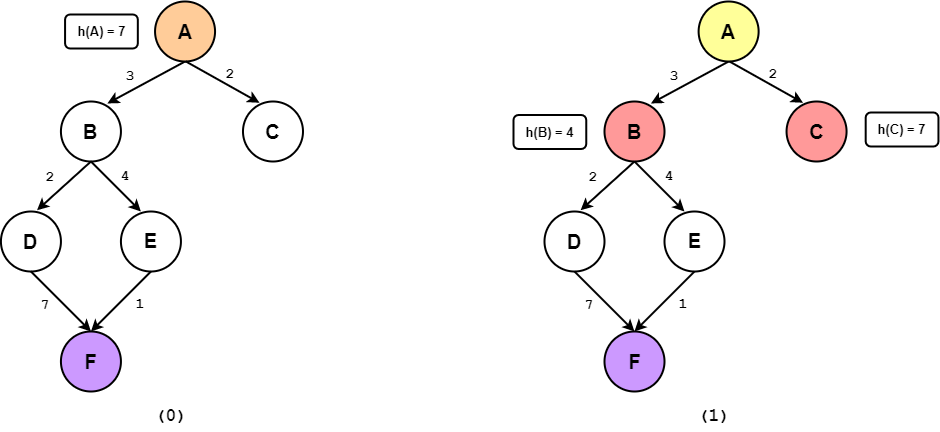
\includegraphics[scale=0.5]{pic/Greedy1.png}
    \label{fig:my_label}
\end{figure}
\begin{figure}[H]
    \centering
    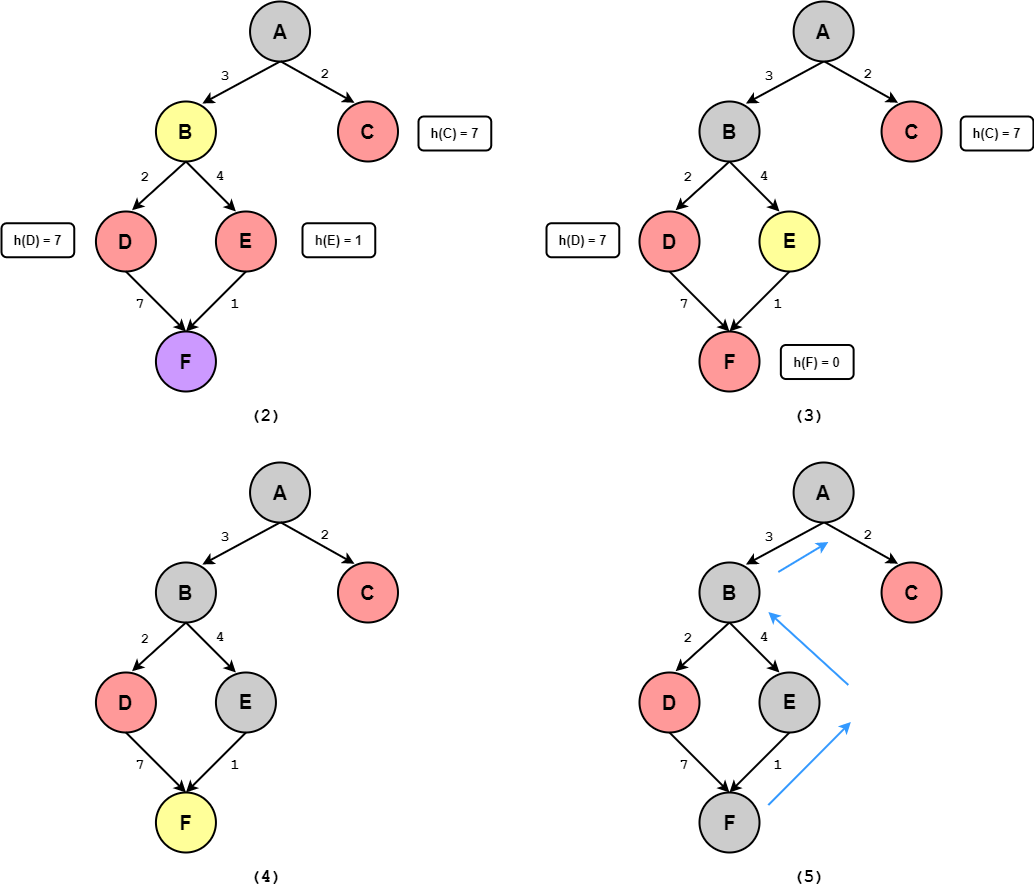
\includegraphics[scale=0.5]{pic/Greedy2.png}
    \label{fig:my_label}
\end{figure}
\begin{table}[H]
{
\renewcommand{\arraystretch}{1}
\centering
\begin{tabular}{|m{1cm}|m{6.4cm}|m{1.6cm}|m{2.6cm}|m{3.3cm}|}
\hline
\begin{center}\cellcolor{green!25}\textbf{Step}\end{center}& \centering\cellcolor{green!25}\textbf{Description} & \centering\cellcolor{yellow!25}\textbf{Current} & \centering\cellcolor{red!25}\textbf{Opened Set\\(Priority Queue)} & \begin{center}\cellcolor{gray!25}\textbf{Closed Set}\end{center} \\ \hline
   \centering 0 & enqueue(A,7) into empty Queue & & \begin{center} \{(A,7)\} \end{center} & \begin{center} \{-\} \end{center} \\ \hline
   \centering 1 & dequeue()= (A,7), enqueue(B,4),\par enqueue(C,7) & \begin{center} (A,7) \end{center}& \begin{center} \{(B,4),(C,7)\} \end{center} &  \begin{center} \{-\} \end{center} \\ \hline
   \centering 2 & A closed, dequeue()= (B,4)\par enqueue(D,7), enqueue(E,1) & \begin{center} (B,7) \end{center}& \begin{center} \{(E,1),(C,7)\par(D,7)\} \end{center} & \begin{center} \{(A,7)\} \end{center}\\ \hline 
   \centering 3 & B closed, dequeue()= (E,1),\par enqueue(F,0) & \begin{center} (E,1) \end{center} & \begin{center} \{(F,0),(C,7),\par(D,7)\} \end{center} & \begin{center} \{(A,7),(B,4)\} \end{center} \\ \hline 
\end{tabular}
}
\end{table}

\begin{table}[H]
{
\renewcommand{\arraystretch}{1}
\centering
\begin{tabular}{|m{1cm}|m{6.4cm}|m{1.6cm}|m{2.6cm}|m{3.3cm}|}
\hline
\centering 4 & E closed, dequeue()= (F,0) =\textbf{ goal} \par Return Path & \begin{center} (F,0) \end{center} & \begin{center} \{(C,7),(D,7)\} \end{center} & \begin{center} \{(A,7),(B,4),(E,1)\} \end{center} \\ \hline 
   \centering 5 & \begin{center}Path A $\rightarrow$ F: A $\rightarrow$ B $\rightarrow$ E $\rightarrow$ F \end{center}&  &  &  \\ \hline 
\end{tabular}
}
\caption*{Các bước tìm kiếm bằng Greedy Best First Search}
\end{table}
\hspace{0.42cm} Để dễ hình dung về ví dụ trên, ta cần lưu ý một số điểm như sau:
\begin{itemize}
    \item Mức độ ưu tiên để lấy ra phần tử nào là giá trị \textbf{$h(x) = $} Ước lượng khoảng cách giữa node đang xét và node đích. 
    \item Cách duyệt cũng tương tự với thuật toán UCS là duyệt theo giá trị nhỏ nhất lấy ra (dequeue) được từ \textbf{Opened Set}.
\end{itemize}

\section{A* Search}
\subsection{Ý tưởng chung}
\hspace{0.42cm} A* Search là một thuật toán tìm kiếm  trong đồ thị. Thuật toán sẽ tìm kiếm đường đi từ đỉnh nguồn đến đỉnh đích sao cho chi phí là thấp nhất và số bước duyệt là ít nhất bắng cách sử dụng hàm để ước lượng khoảng cách hay còn gọi là hàm Heuristic. 

\hspace{0.42cm} A* lưu giữ một tập các lời giải chưa hoàn chỉnh, nghĩa là các đường đi qua đồ thị, bắt đầu từ đỉnh nguồn. Tập lời giải này được lưu trong một hàng đợi ưu tiên (priority queue). Thứ tự ưu tiên được gán cho một đường đi được quyết định bởi hàm $f(x) = g(x) + h(x)$
\begin{itemize}
    \item $g(x)$ là chi phí đường đi từ đỉnh nguồn cho đến đỉnh $x$ hiện tại.
    \item $h(x)$ là chi phí được ước lượng để đến đích từ $x$.
    \item $f(x)$ là chi phí tổng thể ước lượng của đường đi qua đỉnh $x$ hiện tại để đến đích. $f(x)$ có giá trị càng thấp thì độ ưu tiên của $x$ càng cao.
\end{itemize}
\hspace{0.42cm} 

\subsection{Mã giả}

\begin{algorithm}[H]
    \caption{\textbf{Mã giả:} A* Search}
    \begin{algorithmic}[1]
    \Require{
    \begin{tabular}{cl}
    G & Đồ thị cần tìm đường đi\\
    start & Đỉnh bắt đầu\\
    goal & Đỉnh đích\\
    \end{tabular}
    }
    \Ensure{\begin{tabular}{cl}
    Path & Đường đi từ start tới goal (nếu có)\\
    \end{tabular}} 
             \algstore{1}
    \end{algorithmic}
\end{algorithm}
\begin{algorithm}[H]
    \begin{algorithmic}[1]
    \algrestore{1}
    \State \textcolor{cmt}{\Comment{Get distance from start to goal by Euclidean distance}}
    \Function{get\_distance}{$start, goal$}
        \State \Return \textbf{sqrt}$((goal.x-start.x)^2+(goal.y-start.y)^2))$
    \EndFunction
    \Function{get\_heuristic}{$node$}
        \State \Return \textbf{abs}$(goal.x-node.x)$+\textbf{abs}$(goal.y-node.y)$  \textcolor{cmt}{\Comment{Diagonal distance}}
    \EndFunction
    \State \textcolor{cmt}{\Comment{Implement Function}}
    \Function{AStar}{$G,start,goal$}
        \State $open\_set \gets \text{Priority Queue}$ \textcolor{cmt}{\Comment{ (key, value) = (node, fcost), fcost = f(n) = g(n) +h(n)}}
        \State $open\_set.$\textbf{enqueue}$(start,$ \textbf{get\_heuristic}$(start))$
        \While{$open\_set$ is not empty}
            \State \textcolor{cmt}{\Comment{ Removing node which lowest fcost from priority queue}}
            \State $current \gets open\_set.\textbf{dequeue}( )$
             \If{$current$ is $goal$} 
                \State \textbf{return} \text{Path}
            \EndIf
            \State mark $current$ as $closed$
            \State \textcolor{cmt}{\Comment{ Processing all neighbors of current}}
            \For{each $node$ of $current$'s neighbors}
                \If{$node$ is not \textbf{in} $closed$}
                    \State $totalcost \gets gcost[current] + \textbf{get\_distance}(current, node)$
                    \If{node \textbf{ not in } opened\_set}
                        \State $opened\_set. \textbf{enqueue}((node, totalcost + \textbf{get\_heuristic}(node)))$
                    \Else{ \textbf{if} $totalcost < gcost[node]$}
                        \State $gcost[node] \gets totalcost $
                        \State \textcolor{cmt}{\Comment{replace by lower fcost}}
                        \State \text{replace }$(node, fcost)$\text{ with } $(node,totalcost + $\textbf{get\_heuristic}$(node))$ 
                    \EndIf
                \EndIf
            \EndFor
        \EndWhile
        \State \textbf{return} \text{Not found path}
    \EndFunction
    \end{algorithmic}
\end{algorithm}

\subsection{Nhận xét}
\subsubsection{a) Tính đầy đủ}
\hspace{0.42cm} A* Search có tính đầy đủ nếu đồ thị là hữu hạn với chi phí giữa tất cả các cạnh trong đồ thị là không âm. Điều kiện để đảm bảo tính đầy đủ của thuật A* Search tương tự với điều kiện của thuật toán Uniform Cost Search. 
\subsubsection{b) Tính tối ưu}
\hspace{0.42cm} A* Search có tính tối ưu khi hàm heuristic $h(x)$ là \textbf{admissible}, khi đó $h(x)$ phải thỏa: $\forall x$, $ h(x) \leq h^{*}(x)$. Trong đó:
\begin{itemize}
    \item $x$ là 1 đỉnh trong đồ thị.
    \item $h$ là hàm heuristic
    \item $h(x)$ là chi phí được ước lượng bởi $h$ để đến đích từ $x$.
    \item $h^{*}(x)$ là chi phí tối ưu thực tế để đến đích từ $x$
\end{itemize}
Bởi vì $g(x)$ là chi phí thực tế để đi từ đỉnh xuất phát đến đỉnh $x$ hiện tại và $f(x) = g(x) + h(x)$, do đó $h(x)$ phải thỏa mãn điều kiện trên để chi phí ước lượng tổng thể $f(x)$ không vượt quá chi phí tối ưu thực tế của đường đi từ đỉnh xuất phát đến đỉnh đích qua đỉnh $x$.
\subsubsection{c) Độ phức tạp}

\hspace{0.42cm} Độ phức tạp thời gian của thuật toán A{*} Search phụ thuộc vào hàm heuristic được sử dụng. Một hàm heuristic tốt sẽ giúp A{*} loại bỏ nhiều node không cần thiết phải mở rộng thay vì cứ mở rộng hết tất cả các node có thể như các thuật toán uninformed search. Trong trường hợp xấu nhất, hàm heuristic được sử dụng hoàn toàn \textbf{mù} thông tin và kiến thức, khi đó A{*} hoạt động giống như BFS với độ phức tạp = $O(b^d)$, với \textbf{d} = độ sâu của node đích và \textbf{b} = số node tối đa mà 1 node có thể mở rộng

\subsection{Ví dụ}

\begin{figure}[H]
    \centering
    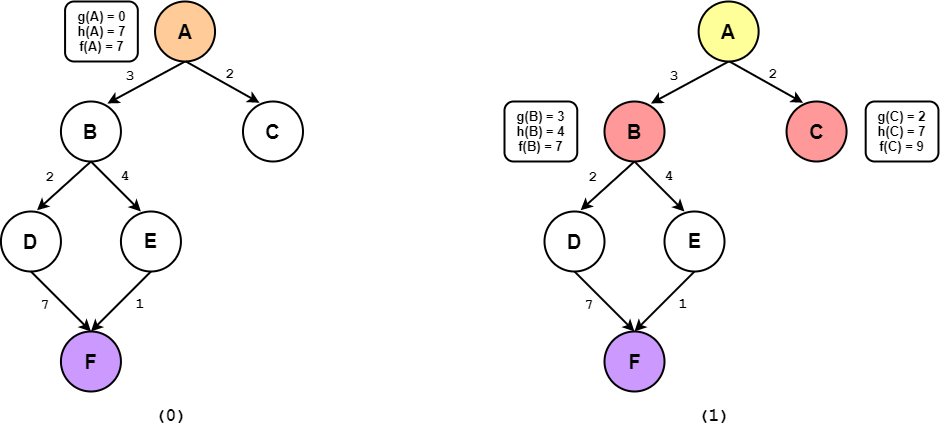
\includegraphics[scale=0.5]{pic/A1.png}
    \label{fig:my_label}
\end{figure}
\begin{figure}[H]
    \centering
    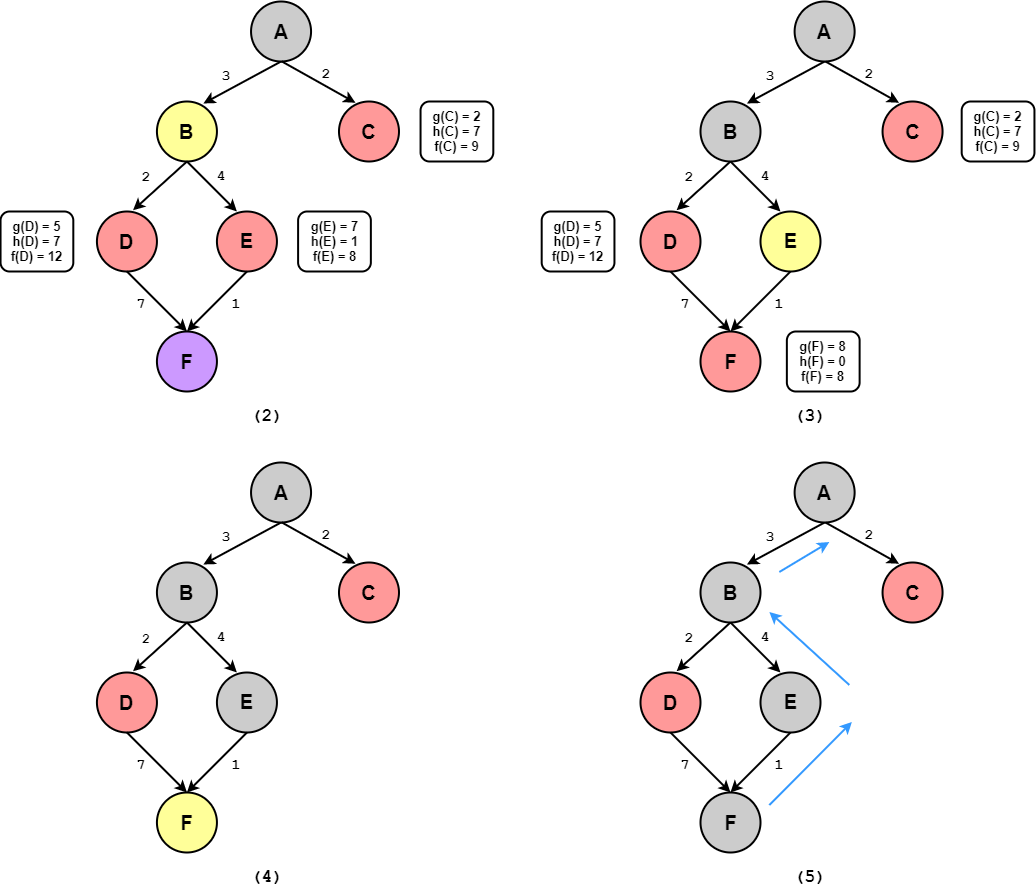
\includegraphics[scale=0.5]{pic/A2.png}
    \label{fig:my_label}
\end{figure}
\begin{table}[H]
{
\renewcommand{\arraystretch}{1}
\centering
\begin{tabular}{|m{1cm}|m{6.4cm}|m{1.6cm}|m{2.6cm}|m{3.3cm}|}
\hline
\begin{center}\cellcolor{green!25}\textbf{Step}\end{center}& \centering\cellcolor{green!25}\textbf{Description} & \centering\cellcolor{yellow!25}\textbf{Current} & \centering\cellcolor{red!25}\textbf{Opened Set\\(Priority Queue)} & \begin{center}\cellcolor{gray!25}\textbf{Closed Set}\end{center} \\ \hline
   \centering 0 & enqueue(A,7) into empty Queue & & \begin{center} \{(A,7)\} \end{center} & \begin{center} \{-\} \end{center} \\ \hline
   \centering 1 & dequeue()= (A,7), enqueue(B,7),\par enqueue(C,9) & \begin{center} (A,7) \end{center}& \begin{center} \{(B,7),(C,9)\} \end{center} &  \begin{center} \{-\} \end{center} \\ \hline
   \centering 2 & A closed, dequeue()= (B,7)\par enqueue(D,12), enqueue(E,8) & \begin{center} (B,7) \end{center}& \begin{center} \{(E,8),(C,9),\par(D,12)\} \end{center} & \begin{center} \{(A,7)\} \end{center}\\ \hline 
   \centering 3 & B closed, dequeue()= (E,8),\par enqueue(F,8) & \begin{center} (E,8) \end{center} & \begin{center} \{(F,8),(C,9),\par(D,12)\} \end{center} & \begin{center} \{(A,7),(B,7)\} \end{center} \\ \hline 
\end{tabular}
}
\end{table}
\begin{table}[H]
{
\renewcommand{\arraystretch}{1}
\centering
\begin{tabular}{|m{1cm}|m{6.4cm}|m{1.6cm}|m{2.6cm}|m{3.3cm}|}
\hline
   \centering 4 & E closed, dequeue()= (F,8) =\textbf{ goal} \par Return Path & \begin{center} (F,8) \end{center} & \begin{center} \{(E,7),(F,12)\} \end{center} & \begin{center} \{(A,7),(B,7),(E,8)\} \end{center} \\ \hline 
   \centering 5 & \begin{center}Path A $\rightarrow$ F: A $\rightarrow$ B $\rightarrow$ E $\rightarrow$ F \end{center}&  &  &  \\ \hline 
\end{tabular}
}
\caption*{Các bước tìm kiếm bằng Greedy Search}
\end{table}

\hspace{0.42cm} Để dễ hình dung về ví dụ trên, ta cần lưu ý một số điểm như sau:
\begin{itemize}
    \item Một vài lưu ý tương tự UCS đã trình bày như ở trên. Đặc biệt mức độ ưu tiên để lấy ra phần tử nào là giá trị $f(x) = g(x) + h(x)$. 
    \item Khi có 2 phần tử có giá trị $f(x)$ bằng nhau thì A* sẽ hoạt động giống như DFS giữa các phần tử đó để tránh khám phá nhiều hơn một giải pháp tối ưu.
\end{itemize}

\chapter{ So sánh các thuật toán}
\section{Sự khác biệt giữa Depth First Search (DFS) và Breadth First Search (BFS)}
\begin{center}
    \begin{tabular}{ |m{3cm}|m{6cm}|m{6cm}|}
    \hline
    \rowcolor[RGB]{229,229,229} 
    \begin{center}\textbf{Tiêu chí so sánh}\end{center} & \begin{center}\textbf{Depth First Search (DFS)}\end{center} & \begin{center}\textbf{Breadth First Search (BFS)}\end{center}  \\ \hline
    \centering Cấu trúc dữ liệu sử dụng & Duyệt lần lượt tất cả các node trên cùng một nhánh cho đến khi không còn đi sâu hơn được nữa, sau đó mới chuyển sang nhánh kế tiếp & Duyệt lần lượt tất cả các node trên cùng mức sau đó mới chuyển sang duyệt mức kế tiếp  \\ \hline
    \centering Bộ nhớ & Ít tốn bộ nhớ hơn & Tốn bộ nhớ hơn \\ \hline
    \centering Thời gian & $O(b^m)$ \par
   - b = số node tối đa mà 1 node có thể mở rộng \par
   - m = độ sâu tối đa & $O(b^s)$ \par
   - b = số node tối đa mà 1 node có thể mở rộng \par
   - s = độ sâu của node đích  \\ \hline
    \centering Tính tối ưu & Không tối ưu & Tối ưu \\ \hline
    \centering Khi nào nên dùng? & Khi node đích ở xa node nguồn, DFS hoạt động tốt hơn & Khi node đích ở gần node nguồn, BFS hoạt động tốt hơn \\ \hline
    \end{tabular}
\end{center}

\section{Sự khác biệt giữa Uniform Cost Search (UCS) và Dijkstra}

\hspace{0.42cm} Cả thuật toán Dijkstra và thuật toán Uniform Cost Search đều có hướng giải quyết bài toán tìm đường đi ngắn nhất tương tự nhau với cùng độ phức tạp về thời gian. Hai thuật toán cũng sử dụng cùng một công thức, $dist[v] = min(dist[v], dist[u] + w(u, v))$, để cập nhật giá trị khoảng cách của mỗi đỉnh.
\begin{center}
    \begin{tabular}{ |m{3cm}|m{6cm}|m{6cm}|}
    \hline
    \rowcolor[RGB]{229,229,229} 
    \begin{center}\textbf{Tiêu chí so sánh}\end{center} & \begin{center}\textbf{Uniform Cost Search (UCS)}\end{center} & \begin{center}\textbf{Dijkstra}\end{center}  \\ \hline
    \centering Cài đặt & Dừng khi tìm được đường đi từ đỉnh nguồn tới đỉnh đích & Dừng khi tìm được đường đi từ đỉnh nguồn tới tất cả các đỉnh còn lại trong đồ thị  \\ \hline
    \centering Yêu cầu về bộ nhớ & Chỉ lưu trữ những đỉnh cần thiết & Phải lưu trữ toàn bộ đồ thị \\ \hline
    \centering Tốc độ chạy & Nhanh hơn vì ít tốn bộ nhớ hơn & Chậm hơn vì tốn bộ nhớ hơn  \\ \hline
    \centering Ứng dụng & Ứng dụng với cả đồ thị tường minh (explicit graph) và đồ thị không tường minh (implicit graph) & Chỉ ứng dụng với đồ thị tường minh (explicit graph) \\ \hline
    \end{tabular}
\end{center}

\section{Sự khác biệt 2 nhóm thuật toán Informed Search và Uninformed Search}

\begin{center}
    \begin{tabular}{ |m{3cm}|m{6cm}|m{6cm}|}
    \hline
    \rowcolor[RGB]{229,229,229} 
    \begin{center}\textbf{Tiêu chí so sánh}\end{center} & \begin{center}\textbf{Informed Search (Heuristic Search / Tìm kiếm dựa trên kinh nghiệm)}\end{center} & \begin{center}\textbf{Uninformed Search (Blind Search / Tìm kiếm mù)}\end{center}  \\ \hline
    \centering Phương pháp tìm kiếm & Sử dụng kinh nghiệm và thông tin biết trước về vấn đề cần giải quyết để xây dựng nên hàm đánh giá hướng dẫn tìm kiếm & Không yêu cầu sử dụng bất kỳ thông tin gì về các đối tượng để có hướng dẫn tìm kiếm mà chỉ đơn thuần xem xét các đối tượng theo một hệ thống nào đó để phát hiện ra đối tượng cần tìm \\ \hline
    \centering Tốc độ tìm kiếm & Tìm kiếm được đường đi nhanh hơn & Tìm kiếm được đường đi chậm hơn  \\ \hline
    \centering Hiệu quả & Hiệu quả hơn khi xét đến chi phí và thời gian. Chi phí phát sinh ít hơn và tốc độ tìm đường đi nhanh hơn & Kém hiệu quả hơn vì chi phí phát sinh nhiều hơn và tốc độ tìm đường đi chậm hơn, điển hình như BFS \\ \hline
    \centering Gợi ý/Đề xuất & Dựa trên hàm đánh giá để đề xuất đường đi & Không có bất kỳ đề xuất nào mà chỉ tiến hành mở rộng cho tới khi tìm được đỉnh đích \\ \hline
    \centering Thuật toán áp dụng & \par
   - Greedy Search \par
   - A* Search & \par
   - Breadth First Search (BFS) \par
   - Depth First Search (DFS) \par
   - Uniform Cost Search (UCS) \\ \hline
    \end{tabular}
\end{center}

\chapter{Cài đặt}
\setcounter{figure}{0}

\section{Kết quả của thuật toán Depth First Search}
\begin{figure}[H]
    \centering
    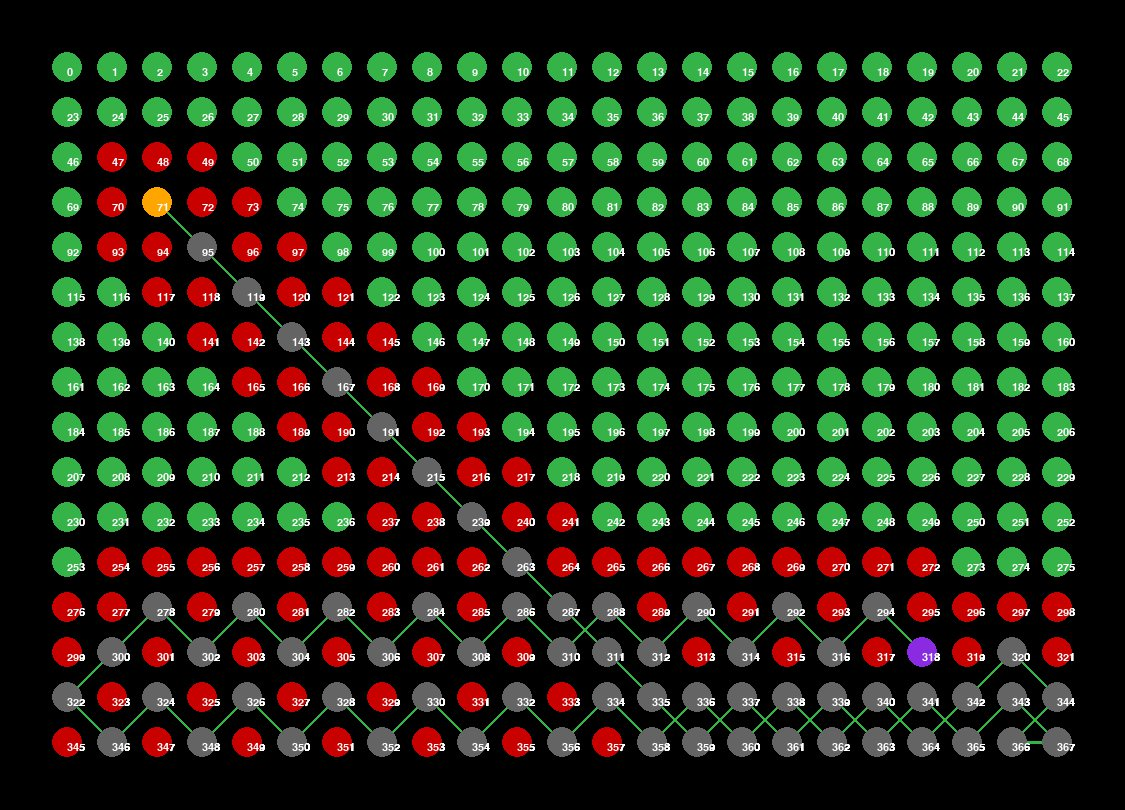
\includegraphics[scale=0.4]{pic/DFS.jpg}
    \label{fig:my_label}
    \caption{Kết quả tìm kiếm của thuật toán Depth First Search}
\end{figure}
\begin{itemize}
    \item \textbf{Mô tả đường đi}: Ta dễ dàng nhận thấy rằng DFS sẽ duyệt về một hướng sâu nhất có thể (71-359) như cái tên của nó. Quá trình đó diễn ra bằng cách phát triển các node lân cận theo chiều sâu. Các node được xét theo thứ tự độ sâu giảm dần cho đến khi tìm được đến đích. Đường đi từ node gốc tới node đích sẽ là quá trình mà thuật toán duyệt lần lượt từng node. 
    \item \textbf{Nhận xét}: 
    \begin{itemize}
        \item Có thể tồn tại nhiều đường đi từ node gốc tới node đích, nhưng DFS luôn trả về kết quả tìm kiếm là đường đi đầu tiên mà nó tìm thấy chứ không quan tâm đến số bước của đường đi đó.
    \end{itemize}
\end{itemize}

\section{Kết quả của thuật toán Breadth First Search}
\begin{figure}[H]
    \centering
    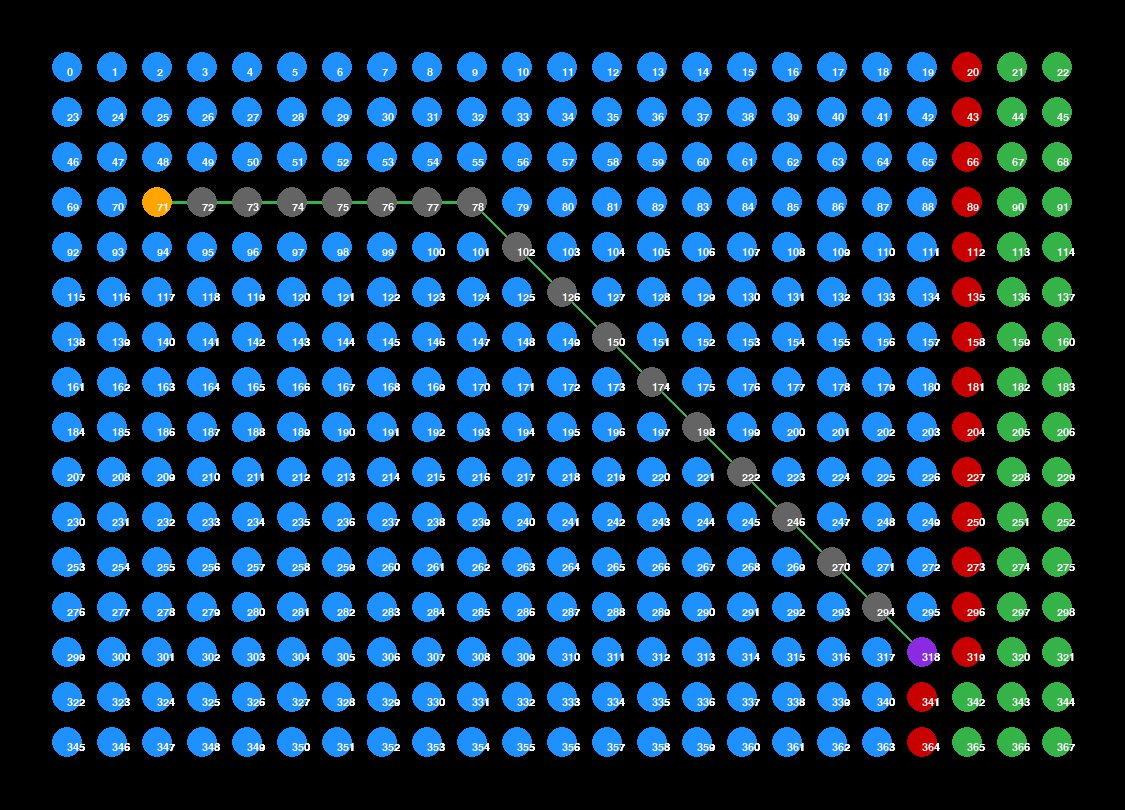
\includegraphics[scale=0.4]{pic/BFS.jpg}
    \label{fig:my_label}
    \caption{Kết quả tìm kiếm của thuật toán Breadth First Search}
\end{figure}
\begin{itemize}
    \item \textbf{Mô tả đường đi}: Ta dễ dàng nhận thấy rằng BFS sẽ duyệt các phần tử xung quanh node gốc. Quá trình đó diễn ra bằng cách phát triển các node lân cận theo chiều rộng. Các node được xét theo thứ tự độ sâu tăng dần cho đến khi tìm được đến đích. Đường đi từ node gốc tới node đích sẽ là đường đi có số bước ngắn nhất có thể.
    \item \textbf{Nhận xét}: 
    \begin{itemize}
        \item Có thể tồn tại nhiều đường đi từ node gốc tới node đích, nhưng BFS luôn trả về kết quả tìm kiếm là đường đi có số bước ngắn nhất có thể. Điều đó đồng nghĩa với việc nếu đồ thị có trọng số bằng nhau thì đây cũng là đường đi có chi phí nhỏ nhất.
    \end{itemize}
\end{itemize}
\section{Kết quả của thuật toán Uniform Cost Search}
\begin{figure}[H]
    \centering
    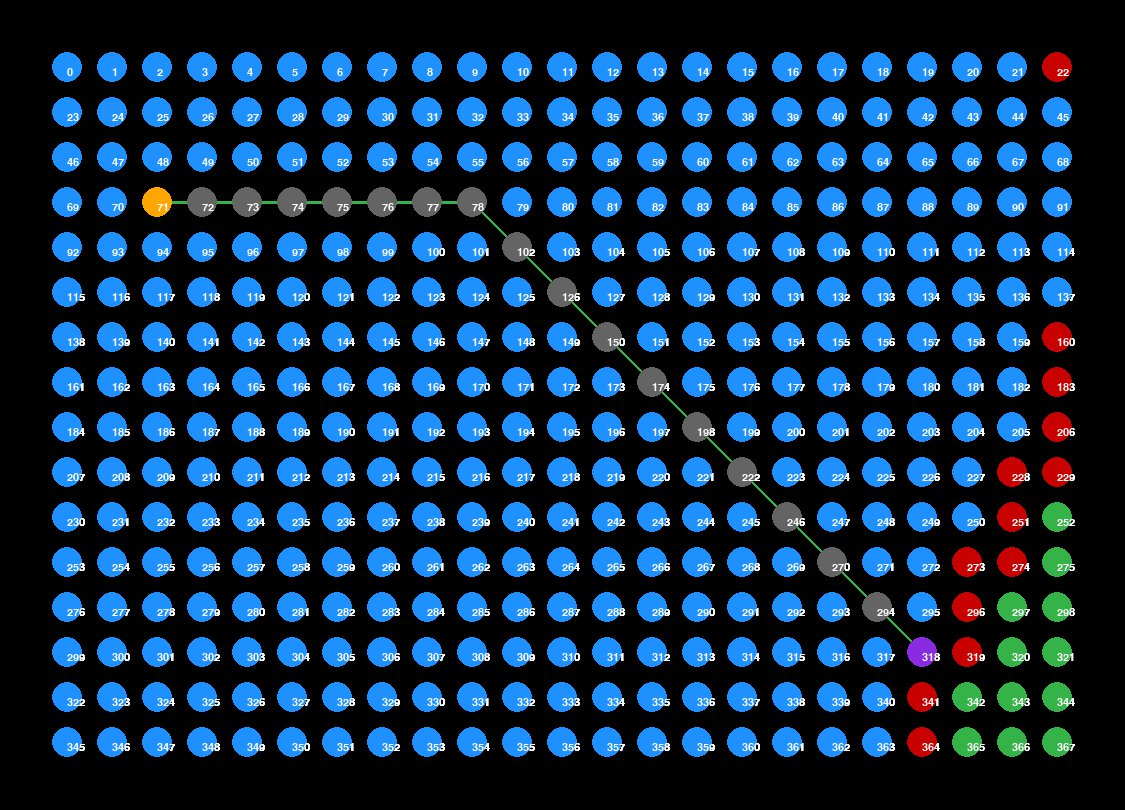
\includegraphics[scale=0.4]{pic/UCS.jpg}
    \label{fig:my_label}
    \caption{Kết quả tìm kiếm của thuật toán Uniform Cost Search}
\end{figure}
\begin{itemize}
    \item \textbf{Mô tả đường đi}: Ta thấy rằng UCS duyệt các phần tử xung quanh node gốc tương tự như cách BFS thực hiện bằng cách phát triển các node lân cận theo chiều rộng. Tuy nhiên các node được chọn để mở rộng không chỉ xét dựa trên chiều rộng mà còn dựa trên chi phí từ node gốc tới node đó, 
    Các node được xét theo thứ tự độ sâu tăng dần cho đến khi tìm được đến đích. Đường đi từ node gốc tới node đích sẽ là đường đi có số bước ngắn nhất có thể.
    \item \textbf{Nhận xét}:
    \begin{itemize}
        \item UCS lựa chọn node tiếp theo để duyệt như cách một ngọn lửa lan rộng ra xung quanh. Nên về cơ bản thì nó khá giống như cách duyệt của BFS, khác ở chỗ BFS duyệt các phần tử lân cận theo một thứ tự nào đó còn UCS lại duyệt dựa vào chi phí thấp nhất.
        \item Ta cũng có thể dễ dàng nhận thấy UCS trả về một một đường đi có chi phí nhỏ nhất nhưng cũng phải bỏ ra rất nhiều thời gian để duyệt và tính toán nhiều lần.
    \end{itemize}
\end{itemize}
\section{Kết quả của thuật toán Greedy Best First Search}
\begin{figure}[H]
    \centering
    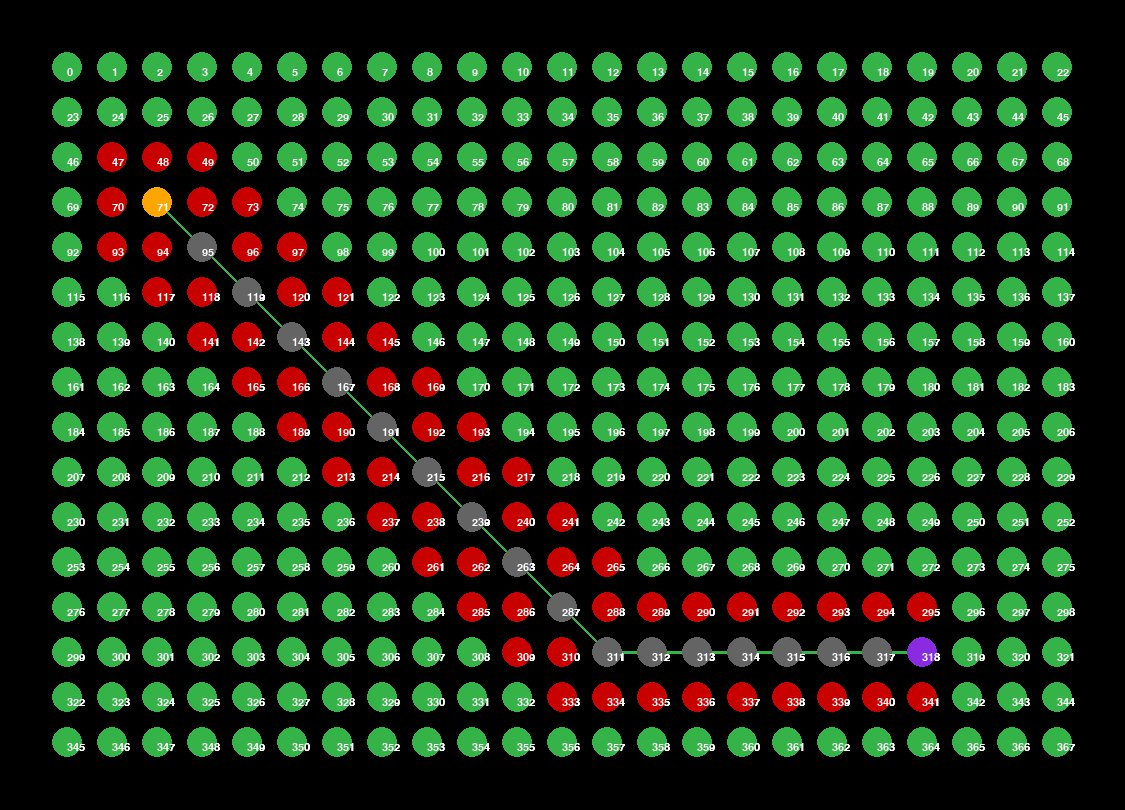
\includegraphics[scale=0.4]{pic/AStar.jpg}
    \label{fig:my_label}
    \caption{Kết quả tìm kiếm của thuật toán Greedy Best First Search}
\end{figure}
\begin{itemize}
    \item \textbf{Mô tả đường đi}: Ở đồ thị này thì thuật toán Greedy BFS dễ dàng tính toán chi phí \textbf{heuristic} để có thể tìm được đường đi ngắn nhất mà không phải duyệt quá nhiều phần tử khác. Hay nói cách khác là vì ta dễ dàng mở rộng các node về 8 hướng khác nhau nên đi chéo sẽ khiến giá trị hàm $h(x)$ giảm rất nhanh. Sau đó khi đến cùng độ sâu với node đích ta chỉ cần đi ngang là tìm được node đích. 
    \item \textbf{Nhận xét}: Giống như cái tên thuật toán, nó \textbf{"tham lam"} tính chi phí tới đích ngay từ đầu mà không quan tâm tới chi phí thực tế. Mặc dù ở đây Greedy tìm ra được đường đi tối ưu tức chi phí nhỏ nhất cho đường đi từ node gốc đến node đích. Nhưng đồ thị ta xét ở đây không có những vật cản như trong thực tế hoặc những node có heuristic rất nhỏ nhưng thực tế lại cần đi rất xa mới tới được đích hoặc đôi khi bị kẹt không thể tìm được tới đích.  
\end{itemize}
\section{Kết quả của thuật toán A* Search}
\begin{figure}[H]
    \centering
    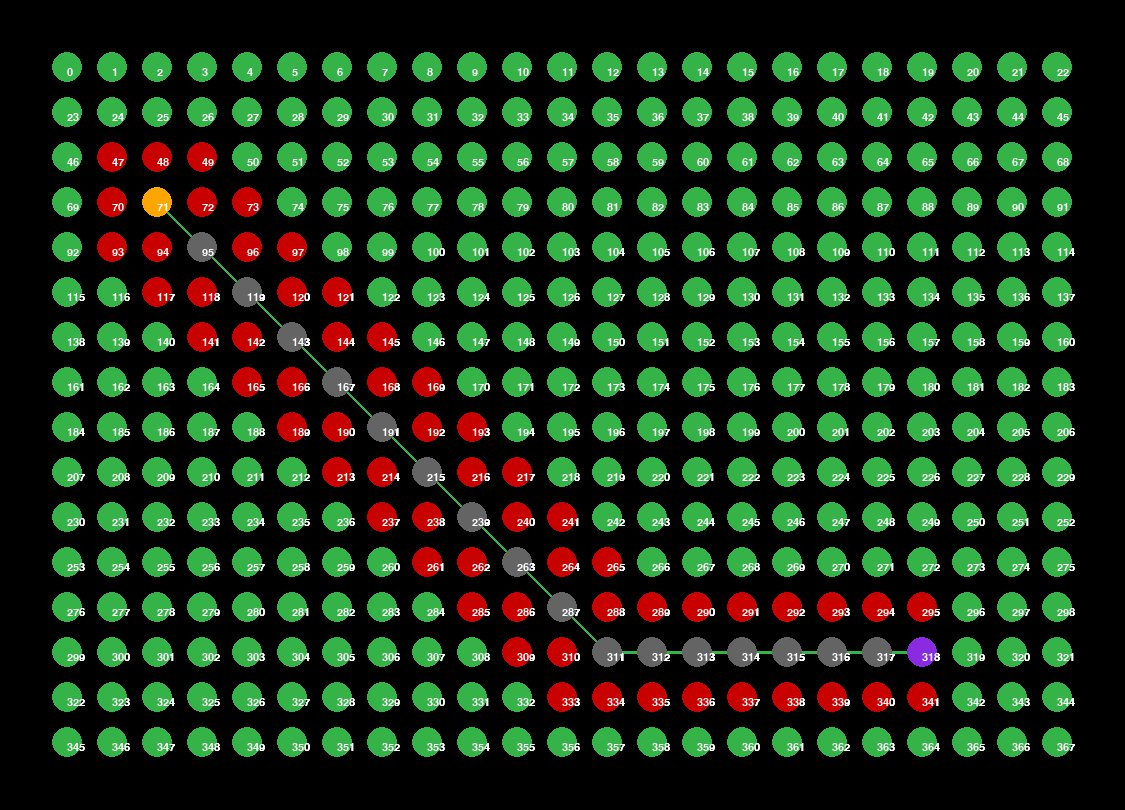
\includegraphics[scale=0.4]{pic/AStar.jpg}
    \label{fig:my_label}
    \caption{Kết quả tìm kiếm của thuật toán A* Search}
\end{figure}
\begin{itemize}
    \item \textbf{Mô tả đường đi}: Là một thuật toán tìm kiếm có kinh nghiệm thì A* đã lựa chọn node tiếp theo để duyệt một cách rất "thông minh". Ban đầu đi theo chiều sâu để $f(x)$ giảm nhanh nhất có thể, khi đến node cùng độ sâu với node đích thì việc đi chéo sẽ có chi phí cao hơn nên A* đã đi \textbf{ngang} để tìm đến đích.
    \item \textbf{Nhận xét}: A* tìm được đường đi có chi phí ngắn nhất mà chỉ phải duyệt rất ít phần tử nhờ kết hợp ưu điểm của cả hai thuật toán UCS và Greedy như đã tìm hiểu ở trên. 
\end{itemize}

\chapter*{\centering Lời kết}\addcontentsline{toc}{chapter}{Lời kết}

 
\hspace{0.42cm}
Trải nghiệm ba tuần thực hiện đồ án: Các thuật toán tìm kiếm trên đồ thị đã giúp chúng em học hỏi được nhiều điều mới mẻ. Từ nguyên lý hoạt động của từng thuật toán tìm kiếm cho đến cách áp dụng chúng vào giải quyết cho từng trường hợp khác nhau, đồng thời chúng em cũng đã có cơ hội rèn luyện thêm những kĩ năng mềm như kĩ năng tự nghiên cứu, tìm kiếm thông tin và làm việc nhóm.\\

\hspace{0.42cm}
Trong quá trình làm việc, do thời gian thực hiên và chỉnh sửa không nhiều cũng như trình độ của nhóm còn có hạn, nên dù chúng em đã rất cố gắng nhưng khó tránh khỏi sai sót xuất hiện. Vì vậy chúng em rất mong nhận được những góp ý và chia sẻ từ quý thầy cô để nhóm có thể cải thiện bài báo cáo, rút kinh nghiệm và thực hiện các đồ án sau này tốt hơn.\\

\hspace{0.42cm}
Chúng em xin chân thành cảm ơn!\\

\begin{minipage}{0.5\textwidth}
\hspace{6cm} \ 
\end{minipage}
\begin{minipage}{0.4\textwidth}
    \begin{center}
    \textbf{Ký tên}\\ \ \\ \ \\

\textbf{Nguyễn Nhật Minh Thư}\\
\textbf{Nguyễn Đặng Anh Thư}
    \end{center}
\end{minipage}

\begin{thebibliography}{9}\addcontentsline{toc}{chapter}{Tài liệu tham khảo}
\bibitem{doc4}
Stuart J. Russell, Peter Norvig, \textit{"Artificial Intelligence: A Modern Approach"}, Third Edition. Prentice Hall, 12-2009.
\bibitem{doc13}
 Nilsson, Nils J.,\textit{"Principles of artificial intelligence"}.Tioga Pub. Co, 1980.
\bibitem{doc14}
Bùi Tiến Lên, \textit{"DSA"}. Truy cập: 25/11/2022 tại \url{https://drive.google.com/drive/folders/0B3x--lrLA0r2a2dhakVwbE5FMUU?resourcekey=0-k4aLP77yxfPIRHwNtWSwug}.
\bibitem{doc1}
John DeNero, Dan Klein, Pieter Abbeel and many others, \textit{"CS188|Introduction to Artificial Intelligence"}. Truy cập: 26/11/2022 tại \url{https://inst.eecs.berkeley.edu/~cs188/fa18/}.
\bibitem{doc3}
GeeksforGeeks, \textit{"Dijkstra’s Shortest Path Algorithm"}. Truy cập: 1/12/2022 tại \url{https://www.geeksforgeeks.org/dijkstras-shortest-path-algorithm-greedy-algo-7/}.
\bibitem{doc5}
GeeksforGeeks, \textit{"Iterative Depth First Search traversal"}. Truy cập: 2/12/2022 tại \url{https://www.geeksforgeeks.org/iterative-depth-first-traversal/?ref=gcse}.
\bibitem{doc6}
GeeksforGeeks, \textit{"Breadth First Search or BFS for a Graph"}. Truy cập: 3/12/2022 tại \url{https://www.geeksforgeeks.org/breadth-first-search-or-bfs-for-a-graph/?ref=gcse}.
\bibitem{doc7}
Fatima Hasan, \textit{"https://www.educative.io/answers/what-is-uniform-cost-search"}. Truy cập: 3/12/2022 tại \url{https://www.educative.io/answers/what-is-uniform-cost-search}.
\bibitem{doc2}
Wikipedia, \textit{"A* search algorithm"}. Truy cập: 3/12/2022 tại \url{https://en.wikipedia.org/wiki/A*_search_algorithm}.
\end{thebibliography}
\end{document}